En esta sección, extenderemos el número de partículas a $N_{part}=1000$, transformando nuestro choque unidimensional en un gas de particulas interactuantes vía potencial
de Pauli: un \textit{gas de Pauli}.
Como dijimos, nuestro objetivo es confirmar si es posible utilizar este potencial para reproducir las distribuciones de un gas de fermiones no interactuantes (o \textit{gas de Fermi}).

El Hamiltoniano de este gas de Pauli será

\begin{equation}{\label{eq:pauli_gas_ham}}
 H(\mathbf{q}_1, ...,\mathbf{q}_N; \mathbf{q}_1,..., \mathbf{q}_N) = \sum_{i=1}^{N} \frac{p_i^2}{2m} + \sum_{i=1}^N\sum_{j=1}^{i-1} De^{-\frac{1}{2}s_{ij}^2}
 \quad \text{ con } \quad s_{ij}^2 = \frac{|\mathbf{q}_i-\mathbf{q}_j|^2}{q_o^2} + \frac{|\mathbf{p}_i-\mathbf{p}_j|^2}{p_o^2}
\end{equation}

\subsection{Método de simulación}

Con esto en mente, comenzamos extendiendo los algoritmos de la Sección \ref{sec:num_choque_1d} para un sistema de $N$ partículas en 3 dimensiones.
En particular, usamos MPR con el método de punto fijo de $k=5$ iteraciones para resolver la ecuación implícita que dicta la evolución temporal del sistema.

Buscamos estimar preliminarmente los tiempos, variando la cantidad de partículas $N$ y analizando el tiempo $\tau_{1000}$ que tardaba el programa en avanzar
$1000$ pasos con $h=5\times10^{-4}$.
Los resultados fueron desalentadores y se encuentran en la \textbf{Figura \ref{}}, donde podemos ver la esperada tendencia cuadrática con 
$\tau_{1000} \approx 0.9753\mu s N^{1.988}$. 
Esto implica que para $N_{part}=1000$, el programa tardaba $\sim0.86s$ por paso, lo cual resulta simplemente prohibitivo al exigir días de simulación para termalizar el sistema.

\begin{figure}[h]
	\centering
	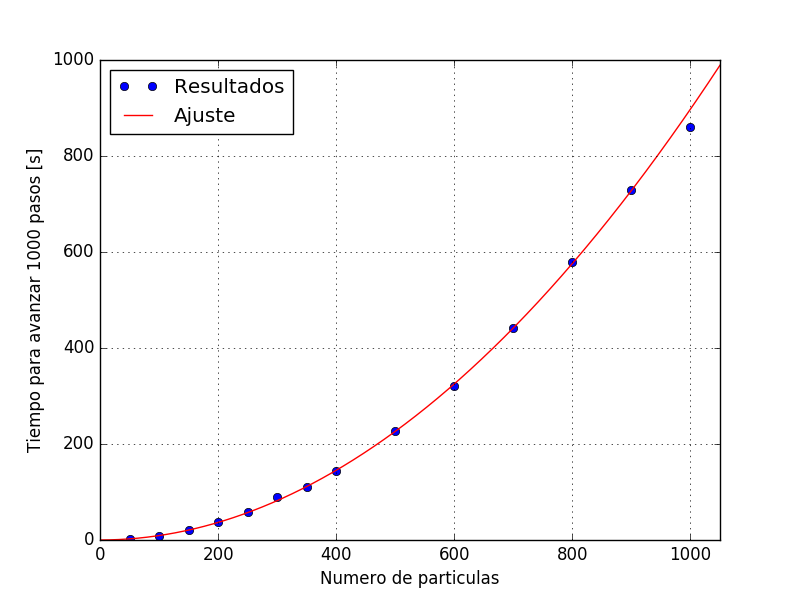
\includegraphics[width=0.6\textwidth]{pauli_gas/tiempo_vs_N.png}
	\caption{Tiempo necesario para avanzar un sistema de $N$ partículas en 1000 pasos con $h=5\times10^{-4}$. 
	La tendencia es cuadrática y exige $\sim0.86s$ por paso para $N=1000$, lo cual es prohibitivo.}
	\label{fig:ej_diag_fases}
\end{figure}

Esto no debería sorprendernos, dado que el método MPR resuelto por punto fijo exige el cómputo de fuerzas $k=5$ veces en total, más del doble de lo exigido por métodos clásicos como Velocity-Verlet.
Además, cabe aclarar que deben computarse las \textit{güerzas} en adición a las fuerzas habituales.
Por último, se suman las complejidades propias del potencial en si, que exige no solo el cálculo de la distancia en el espacio sino también el de la distancia en impulsos y de la necesidad 
de computar una exponencial, siempre más costoso computacionalmente que cualquier potencia. 

Incluso este $k=5$ resultaba insuficiente a medida que $N$ aumentaba, lo cual es razonable si consideramos que la velocidad de convergencia del método de punto fijo (sección \ref{sec:imp_integs})
depende de $N$ a través de $\nabla^2H$.
De hecho, debió tomarse $h=5\times10^{-4}$ (la mitad que en las simulaciones del choque 1D) para mantener la estabilidad del algoritmo durante estras pruebas, lo cual indirectamente exige una 
mayor cantidad de pasos para alcanzar un equilibrio y muestrear propiedades del sistema. 

Frente a esto, consideramos más apropiado el uso del método de Metropolis-Montecarlo descripto en \ref{sec:alg_mm} para el Hamiltoniano \eqref{eq:pauli_gas_ham}.
La principal ventaja de este método es que resulta lineal en $N$ dado que el cómputo de $\Delta E$ al modificar la $k$-esima partícula es

\begin{equation}{\label{eq:delta_E}}
 \Delta E =  \frac{|\mathbf{p}_k + \Delta \mathbf{p}|^2}{2m} - \frac{p_k^2}{2m} + \sum_{i=1, i\neq k}^N D\left( e^{-\frac{1}{2}s_{ik}^{'2}}-e^{-\frac{1}{2}s_{ik}^2}  \right)
\end{equation}

Sin embargo, aún avanzando $N$ pasos (en promedio, un intento de movimiento por partícula) este método tardaba aproximadamente $\tau_N = 0.4s$; menos de la mitad.
Esto sumado a la facilidad para controlar la temperatura (dado que nos interesa un sistema NVT), inclinó la balanza en pos de este método.

En lo que sigue, utilizamos el método de Metropolis-Montecarlo para simular una caja de lado $L$ (y volumen $V=L^3$) con $N$ partículas interactuando mediante un potencial de Pauli $V_P$.
Tomamos valores de $\Delta q$ y $\Delta p$ que nos aseguren una aceptación entre $30\%$ y $60\%$.
Estos $\Delta q$ y $\Delta p$ resultan dependientes de la temperatura $T$, la densidad $\rho = N/V = N/L^3$ e incluso de los propios parámetros del Hamiltoniano.
La forma general de estas variaciones fue entonces $\Delta x = x_o f_x(T, \rho, D^*)$  con $x=q,p$.

Además, impusimos una distancia de corte en el espacio de fases $s_{cut}^2=10$ tal que $V_P=0$ si $s_{ij}\geq s_{cut}$.
Esto lo logramos mediante un \textit{shift} del potencial
\[ V_P(s_{ij}^2) = \left\{\begin{matrix} D(e^{-\frac{1}{2}s_{ij}^2}-e^{-\frac{1}{2}s_{cut}^2}) & \text{si } s_{ij}\leq s_{cut} \\ 0 & \text{si } s_{ij}\geq s_{cut} \end{matrix}\right. \]
donde $e^{-\frac{1}{2}s_{cut}^2}\approx 6.7\times10^{-3}\sim 1\%$ del máximo de interacción para $s_{cut}^2=10$.

Tomamos un sistema con condiciones de contorno periódicas (PBC) y utilizamos el criterio de mínima imagen, para lo cual resultaba necesario que el tamaño $L$ de la caja cumpla
\[ L >2 s_{cut}q_o \approx 6.32q_o \]
de forma tal que no sea posible la interacción con más de una imagen simultaneamente. 

En lo que sigue, analizaremos propiedades de un gas de Pauli bajo dos conjuntos de parámetros habitualmente utilizados en la literatura para Pauli.
En ambos casos, tomaremos una masa $m=100m_p$ con $m_p=938MeV/c^2$ la masa del protón; un elección arbitraria y, en el fondo, no más que una variación del $D^*$.

El primero de estos conjuntos de parámetros corresponde a Dorso \textit{et al} con
\begin{equation}{\label{eq:params_dorso}}
 \begin{matrix}
  p_o = 2.067 MeV\times 10^{-22}s/fm (= 61.969 MeV/c) & q_o = 6 fm\\
  D = \left(\frac{\hbar}{q_op_o}\right)^3 34.32MeV = \left(\frac{1}{1.88}\right)^3 34.32MeV = 5.165MeV & D^* = 126.16
 \end{matrix}
\end{equation}
y el segundo a Maruyama \textit{et al}
\begin{equation}{\label{eq:params_maruyama}}
 \begin{matrix}
  p_o = 120 MeV/c & q_o = 1.644 fm\\
  D = \left(\frac{\hbar}{q_op_o}\right)^3 207MeV = 207MeV & D^* = 1348.375
 \end{matrix}
\end{equation}

En comparación con \eqref{eq:params_dorso}, los parámetros de \eqref{eq:params_maruyama} generan un potencial de mucho mayor intensidad pero con un alcance mucho mayor en $p$
respecto a su alcance en $q$.
Además, tiene un $D^*$ casi 11 veces mayor, pero tiene un área excluída muy similar
\[ A_M\sim 45\hbar \qquad \text{ vs } \qquad  A_D\sim 28\times1.88\hbar \sim 52\hbar\]
Cualquier diferencia entre ambos, entonces, se deberá a cuestiones morfológicas del área excluída definidas por sus $D^*$ tan distintos.
El resto serán cuestiones de escala definidas por $q_o$ y $p_o$.

Analizamos estos parámetros para 3 densidades distintas, pero dado que el $q_o$ de \eqref{eq:params_dorso} resulta casi 4 veces mayor al de \eqref{eq:params_maruyama}, decidimos mantener
constantes las \textit{densidades reducidas} $\rho^* = q_o^3\rho$.
Elegimos entonces $\rho_o^* = (3/2)^3 = 3.375 $, $\rho_1^* = 1 $ y $\rho_2^* = (1/2)^3 = 0.125 $ representando densidades altas, intermedias y bajas, respectivamente.
Enfriamos estos sistemas desde una $T$ inicial alta (dependiente de $p_o$) donde esperabamos que el sistema se comporte como un gas ideal y enfriabamos sucesivamente para observar los
efectos termodinámicos del potencial de Pauli.

Finalmente, hicimos simulaciones similares para un gas interactuando mediante un potencial de Lennard-Jones (LJ)
\[ V_{LJ}(r) = \varepsilon\left( \left( \frac{\sigma}{r} \right)^{12} - \left( \frac{\sigma}{r} \right)^6 \right) \]
cuya única dependencia proviene de 2 parámetros $\sigma$ y $\varepsilon$, lo cual nos permite facilmente trabajar en unidades reducidas donde $\sigma=1=\varepsilon=m$.
Analogamente, analizaremos las densidades $\rho_{LJ,1}^* = 1.05$ y $\rho_{LJ,2}^* = 0.4$ representando densidades altas y bajas, respectivamente.

Elegimos estas densidades en base al conocido diagrama de fases del potencial de Lennard-Jones, que nos aseguran que corresponden a gas+líquido, líquido+sólido y sólido.

\begin{figure}[h]
	\centering
	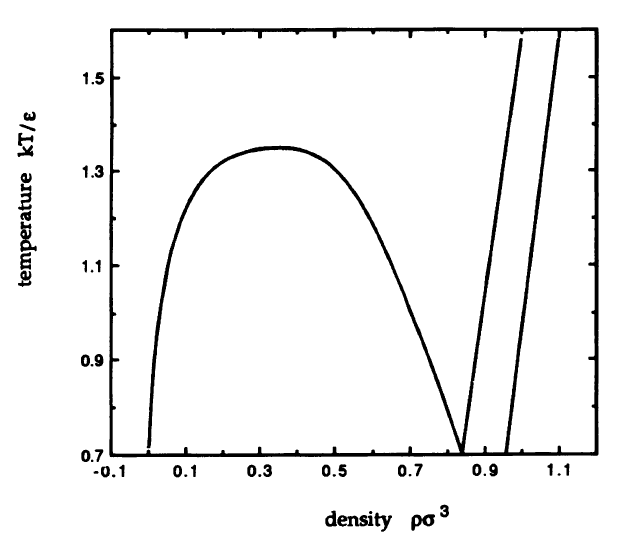
\includegraphics[width=0.4\textwidth]{pauli_gas/phase_diagram_LJ.png}
	\caption{Diagrama de fases de un gas interactuando mediante Lennard-Jones. 
	Esto nos asegura que las densidades elegidas $\rho_{LJ,1}^* = 1.05$ y $\rho_{LJ,2}^* = 0.4$ corresponden a líquido+sólido y gas+líquido.}
	\label{fig:ej_diag_fases}
\end{figure}

Usaremos estas simulaciones a modo de control, para poder apreciar mejor la fenomenología introducida por el potencial de Pauli.
Sin más preambulos, a continuación se encuentran los resultados.


\subsection{Distribución de impulsos}

El enfriamiento se realizó reduciendo la temperatura por etapas, esperando a que termalizara en la nueva temperatura y posteriormente muestreando el estado 
$(\mathbf{q}_1, ..., \mathbf{q}_N;\mathbf{p}_1, ..., \mathbf{p}_N)$ del sistema (las $6N$ coordenadas).
Este proceso de enfriamiento+muestreo se realizó 8 veces en total, inicializando distintas semillas, para tener una mayor cantidad de muestras y mayor descorrelación entre ellas.
En total, se tomaron $200\times 8 = 1600$ muestras del sistema para cada temperatura.

Con toda esa información, hicimos los histogramas de energía cinética del Pauli gas y los comparamos con las distribuciones de Maxwell-Boltzmann (MB) y Fermi-Dirac (FD)
a esa misma $T$ y $\rho$ y con la misma masa $m$, según las ecuaciones \eqref{eq:dist_MB} y \eqref{eq:dist_FD}, respectivamente.

Comenzando con los parámetros \eqref{eq:params_dorso}, vemos los histogramas de las 3 densidades en las \textbf{Figuras \ref{fig:hist_rho0_dorso}}, 
\textbf{\ref{fig:hist_rho1_dorso}} y \textbf{\ref{fig:hist_rho2_dorso}} para algunas temperaturas seleccionadas.
Las comparamos con las distribuciones de MB \eqref{eq:dist_MB} y FD \eqref{eq:dist_FD} correspondientes a esa temperatura $T$ y densidad $\rho$.
También incluimos un ajuste por la distribución de FD \eqref{eq:dist_FD} pero dejando $T$ y $\mu$ como parámetros libres del ajuste.
Esto último equivale a decir que el gas de Pauli se comporta como un gas de Fermi a otra $T'$ y $\rho'$.

\begin{figure}[H]
	\centering
	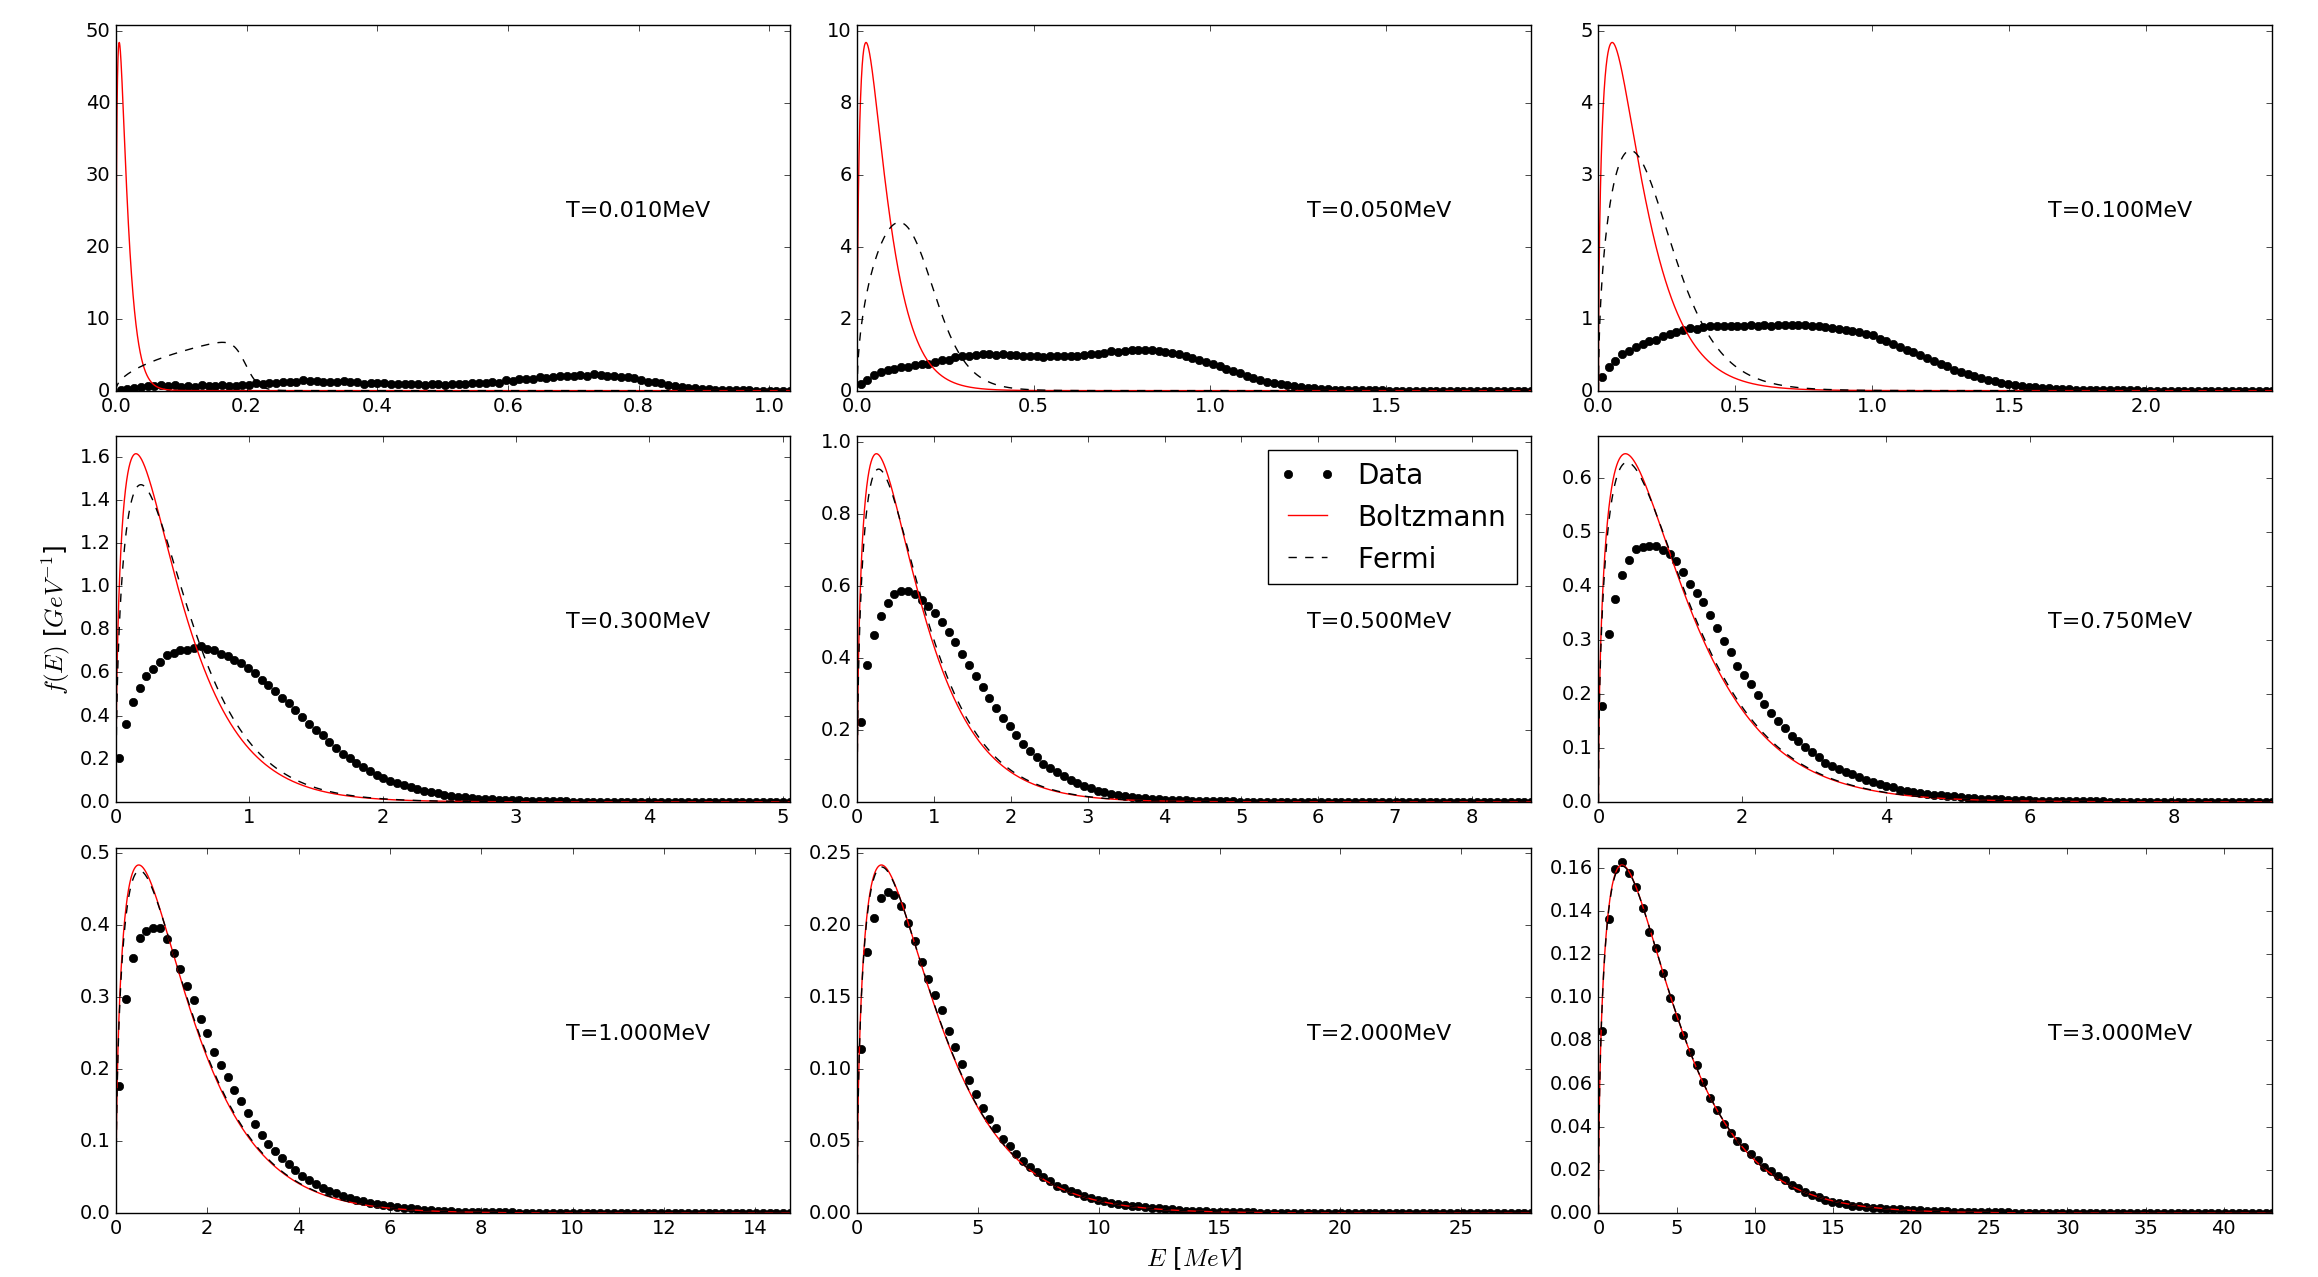
\includegraphics[width=0.9\textwidth]{pauli_gas/hist_rho0_dorso.png}
	\caption{Distribuciones de energía cinética para los parámetros de Dorso en \eqref{eq:params_dorso} y $\rho^* = \rho_o^* = 3.375$}
	\label{fig:hist_rho0_dorso}
\end{figure}

\begin{figure}[H]
	\centering
	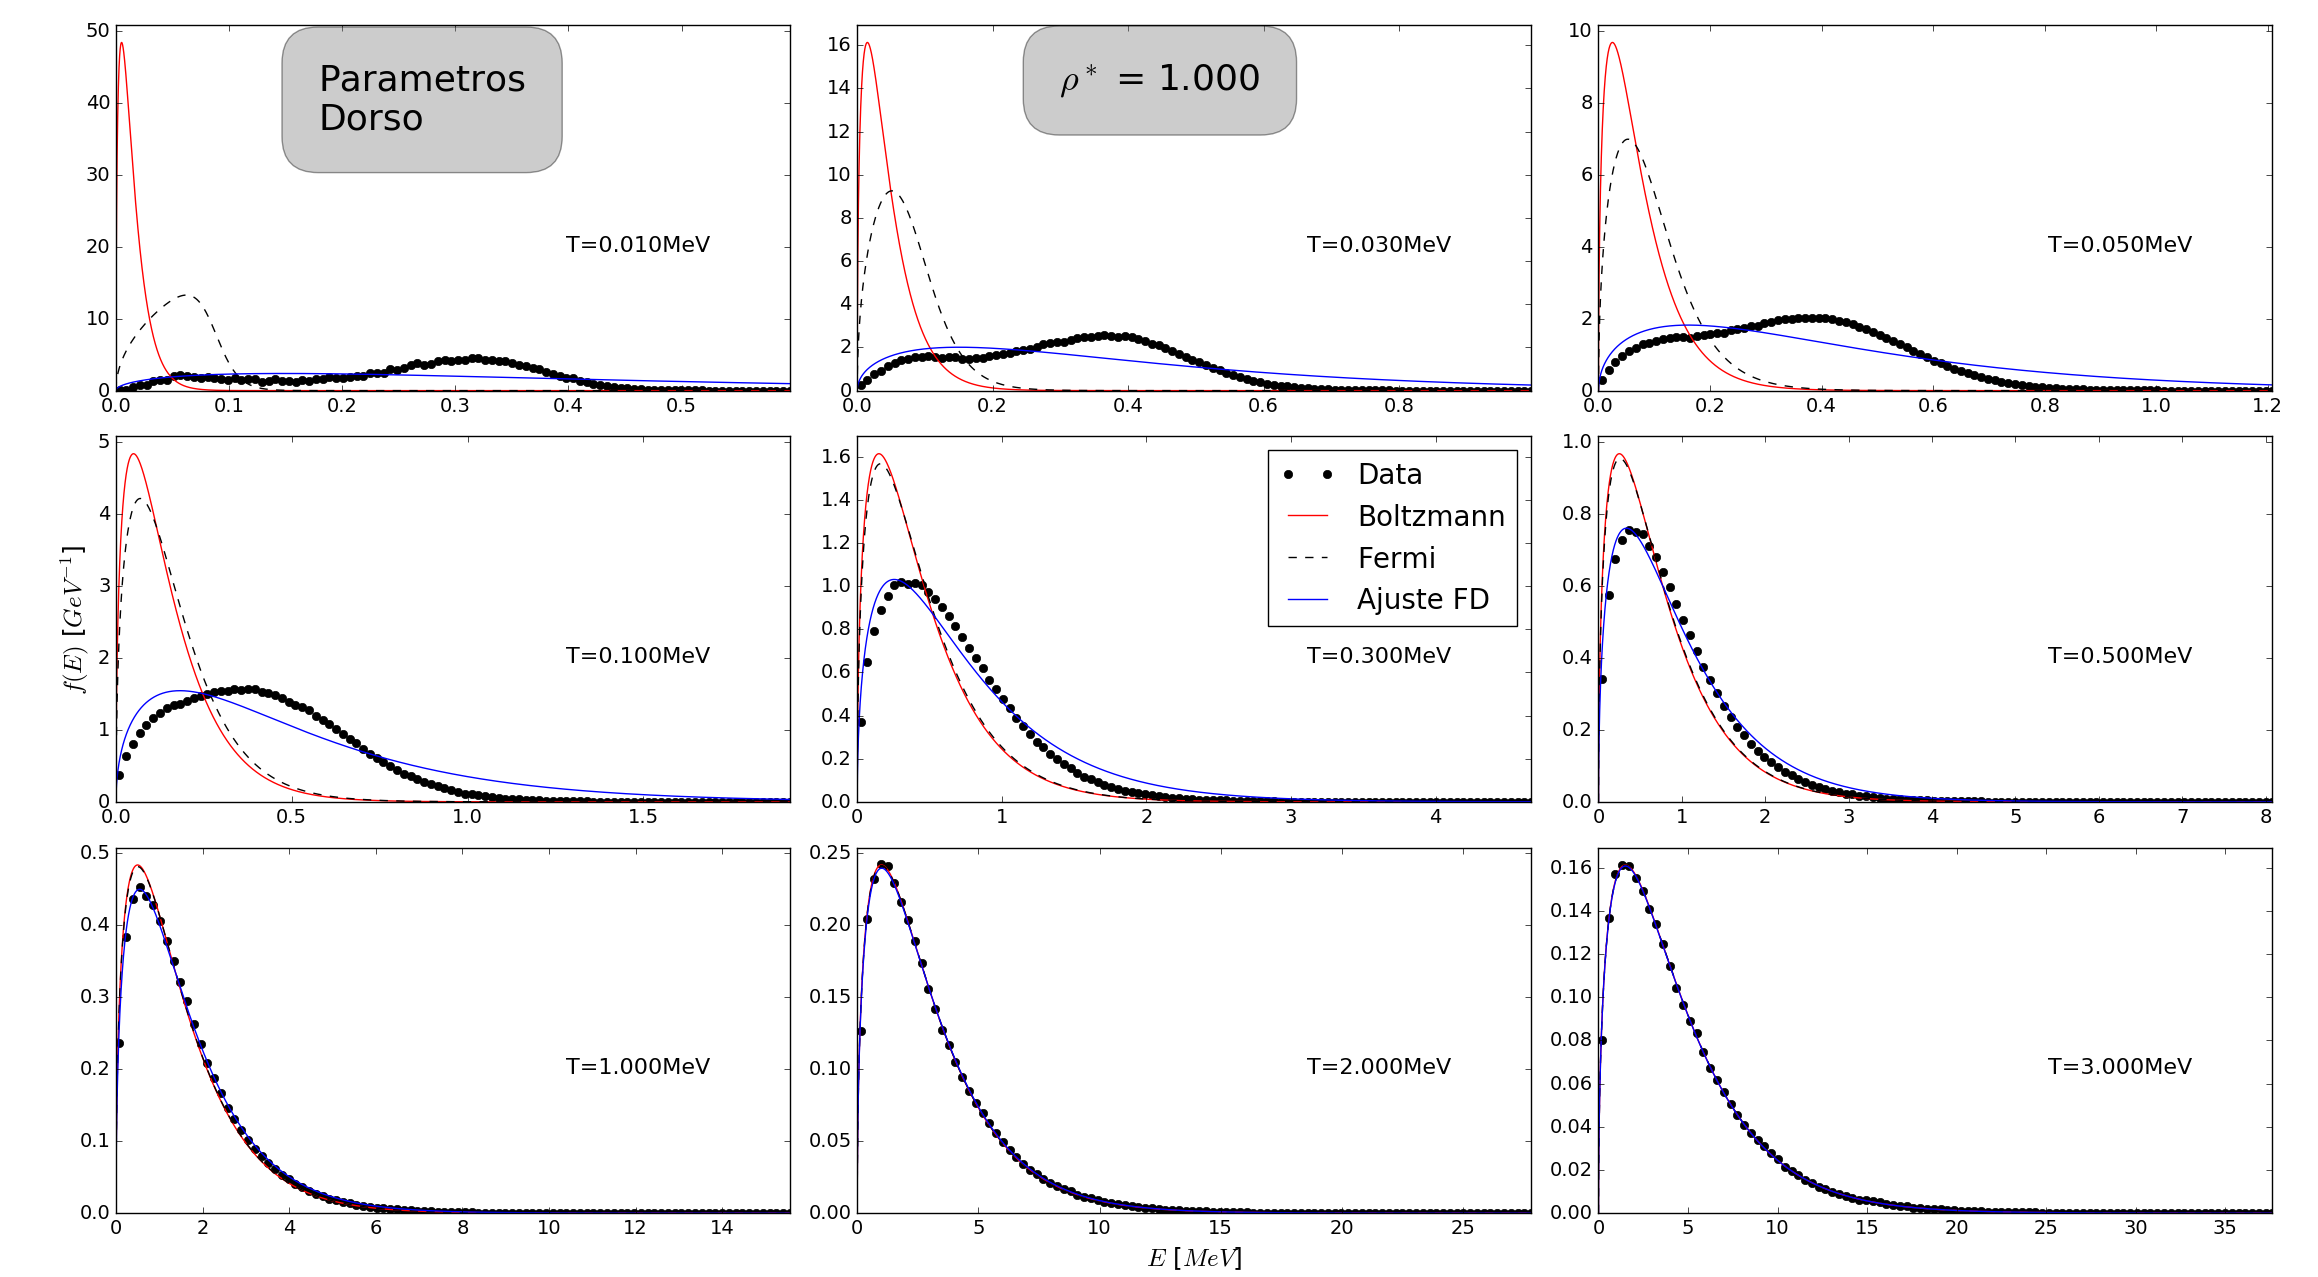
\includegraphics[width=0.9\textwidth]{pauli_gas/hist_rho1_dorso.png}
	\caption{Distribuciones de energía cinética para los parámetros de Dorso en \eqref{eq:params_dorso} y $\rho^* = \rho_1^* = 1$}
	\label{fig:hist_rho1_dorso}
\end{figure}
\begin{figure}[H]
	\centering
	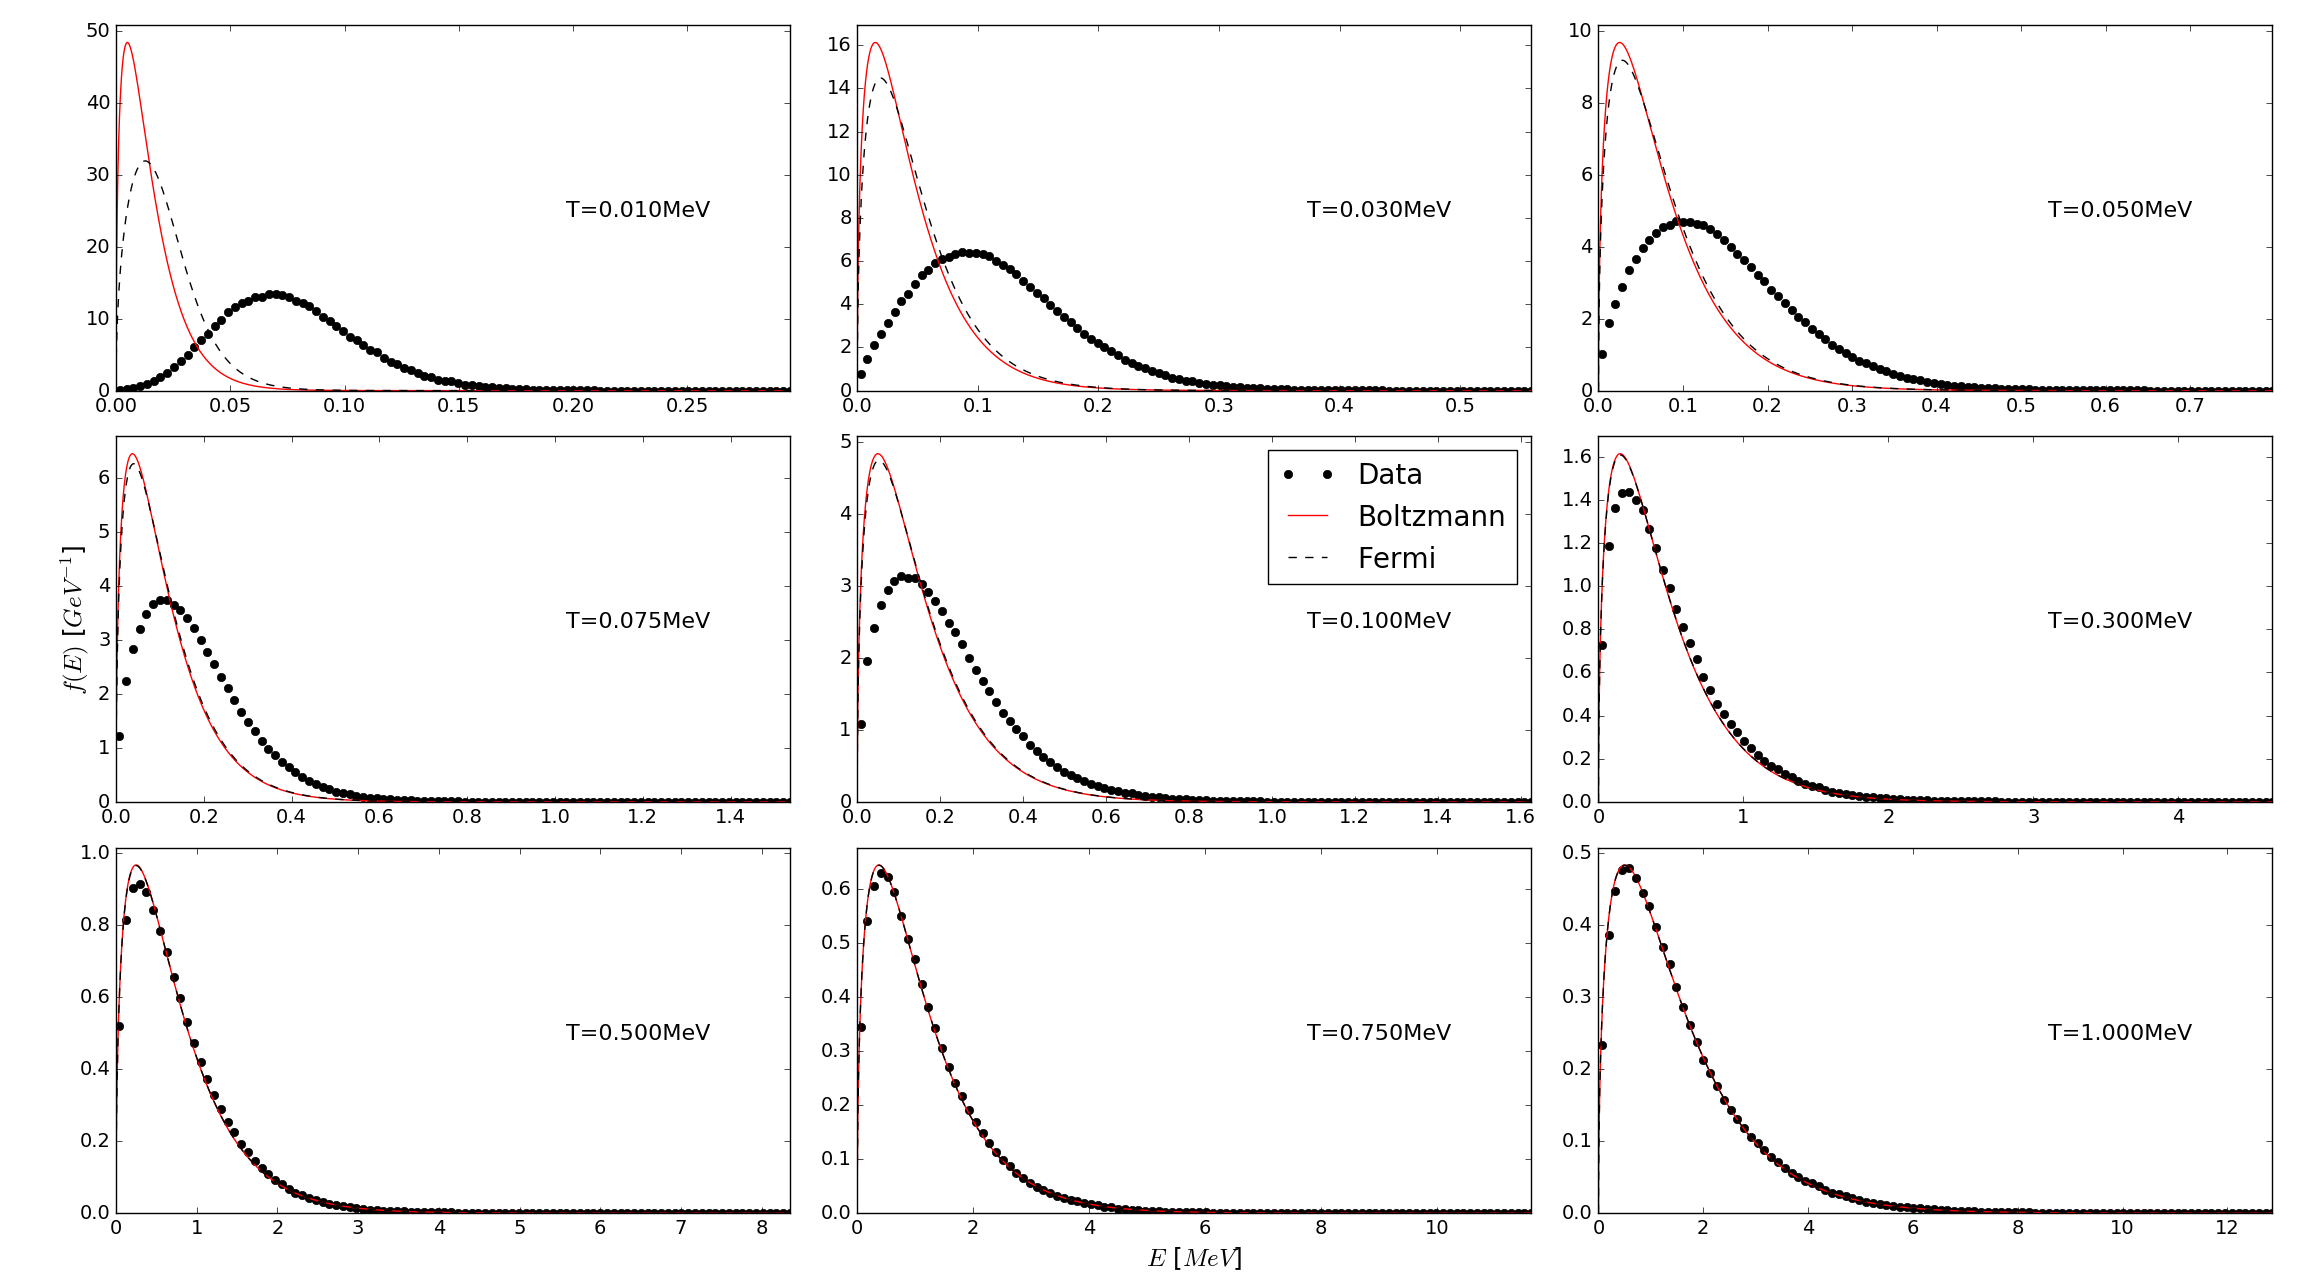
\includegraphics[width=0.9\textwidth]{pauli_gas/hist_rho2_dorso.png}
	\caption{Distribuciones de energía cinética para los parámetros de Dorso en \eqref{eq:params_dorso} y $\rho^* = \rho_2^* = 0.125$}
	\label{fig:hist_rho2_dorso}
\end{figure}

En los 3 casos, podemos apreciar como la distribución se aleja de MB a medida que la temperatura desciende según lo esperado.
Sin embargo, esta separación comienza a una temperatura mayor que la separación de FD respecto a MB.
De hecho, los datos no tienden a acercarse a FD luego de alejarse de MB; solo hay coindicencia de las 3 distribuciones (simultaneamente) a $T$ alta.
Similar a FD, el pico del histograma de los datos no parece acercarse al origen, una de las principales diferencias con MB.
Sin embargo, este pico se da para energías cinéticas mucho mayores que el de FD, lo cual hace pensar que este gas de Pauli sobreestima la exclusión entre las particulas, alejándolas
más de lo que debería.

Más particularmente, podemos notar que la distribución a $T$ baja para $\rho_o^*$ y $\rho_1^*$ tiene 2 picos en lugar de uno, lo cual es muy llamativo.
Para $\rho_2^*$, solo hay un máximo, pero la curva entre este máximo y el origen es cóncava en lugar de convexa a diferencia tanto de MB como FD como de las otras densidades.
Además, la separación de los datos respecto a MB se da a temperaturas cada vez menores a medida que aumentamos $\rho^*$, lo cual también ocurre con FD.
Esto es razonable, dado que la noción de temperatura alta está muy asociada a la de densidad baja como discutimos en \ref{sec:intro_fermi_gas}.

Por el lado de los ajustes, los resultados son prometedores principalmente para temperaturas intermedias; temperaturas para las cuales FD y MB aún no difieren tanto.
Esto nuevamente depende de $\rho$, pues los ajustes son razonablemente acertados para $T\geq 0.5MeV$ en el caso $\rho^*=3.375$, $T\geq 0.3MeV$ para $\rho^*=1$ y $T\geq 0.1MeV$ para $\rho^*=0.125$.
Los gráficos de las \textbf{Figuras \ref{fig:muvsT_dorso}} y \textbf{\ref{fig:TvsT_dorso}} muestran la dependencia de los parámetros ajustados con la temperatura $T$ y la densidad reducida $\rho^*$.
Dado que los gráficos de la \textbf{Figura \ref{fig:muvsT_dorso}} muestran que el $\mu$ de FD tiende a la energía de Fermi $E_F\equiv \mu(T=0,\rho)$, confirmamos que en todos los casos alcanzamos 
el régimen de bajas temperaturas. 
Más allá de esto, notamos que para $T$ alta, ambos $\mu$ coinciden, lo cual es razonable dado que estamos en MB, pero en general es $\mu_{aj}\leq\mu_{FD}$.
A pesar de que la coincidencia para $\rho^*=3.375$ es practicamente inexistente, para $\rho^*=0.125$ esta coincidencia se da en todo el rango de $T$ estudiado.
Algo muy similar ocurre para la $T_{aj}$, que resulta siempre levemente superior a $T$.
Es justamente este $T_{aj}$ quien marca la diferencia entre el ajuste por FD y el FD exacto para $\rho^*=0.125$ donde $\mu_{aj}\approx\mu_{FD}$.

Estas propiedades marcan los dos defectos de Pauli respecto a FD; $T_{aj}\geq T$ implica que la cola de la distribución se extiende para $E$ mayores mientras que $\mu_{aj}\leq\mu_{FD}$ tiende a
desplazar el máximo de la distribución. 

\begin{figure}[H]
	\centering
	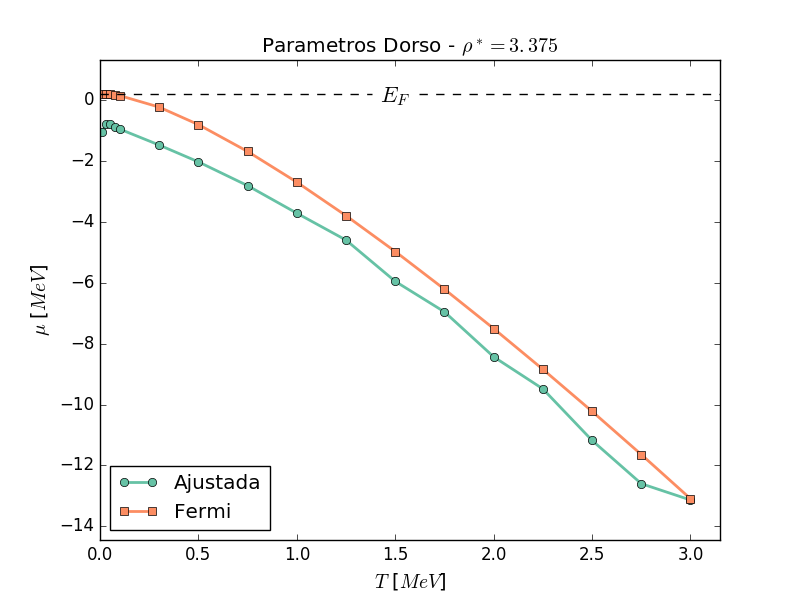
\includegraphics[trim = 5mm 0mm 20mm 5mm, clip, width=0.33\textwidth]{pauli_gas/muvsT_rho0_dorso.png}
	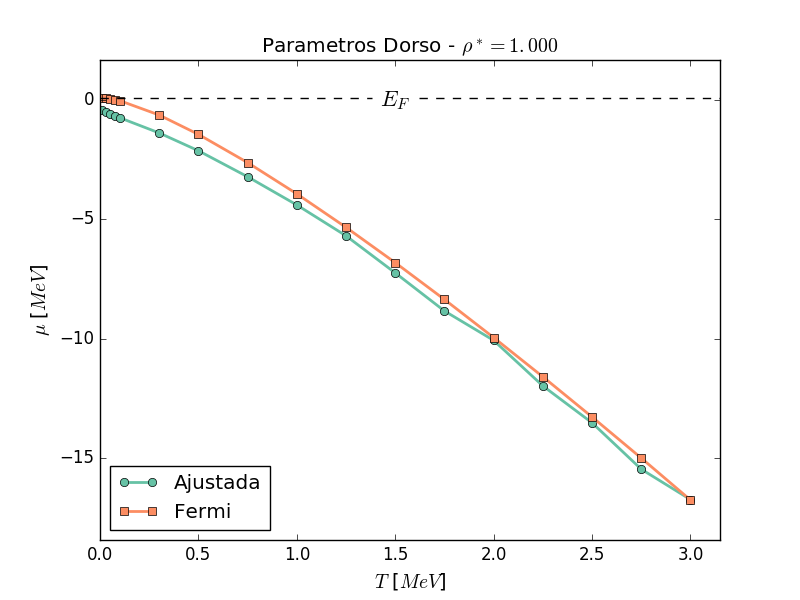
\includegraphics[trim = 5mm 0mm 20mm 5mm, clip, width=0.33\textwidth]{pauli_gas/muvsT_rho1_dorso.png}
	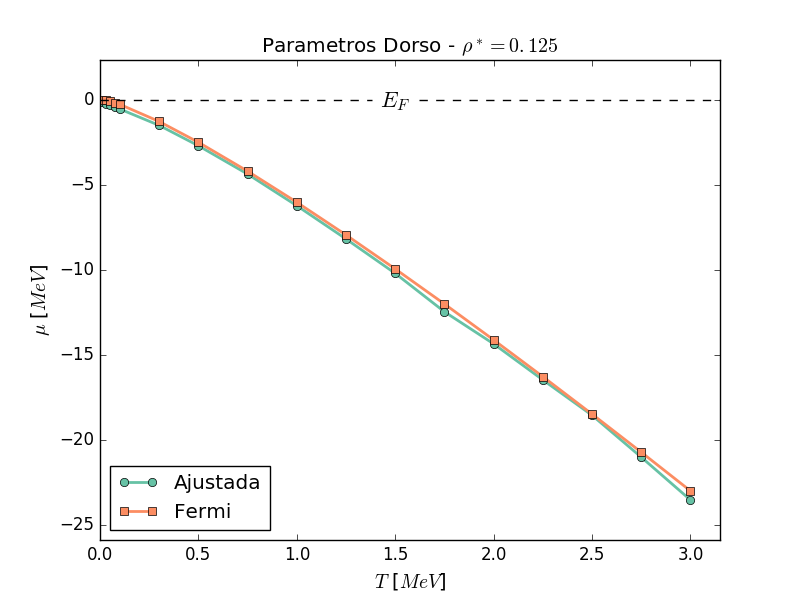
\includegraphics[trim = 5mm 0mm 20mm 5mm, clip, width=0.33\textwidth]{pauli_gas/muvsT_rho2_dorso.png}
	\caption{}
	\label{fig:muvsT_dorso}
\end{figure}
\begin{figure}[H]
	\centering
	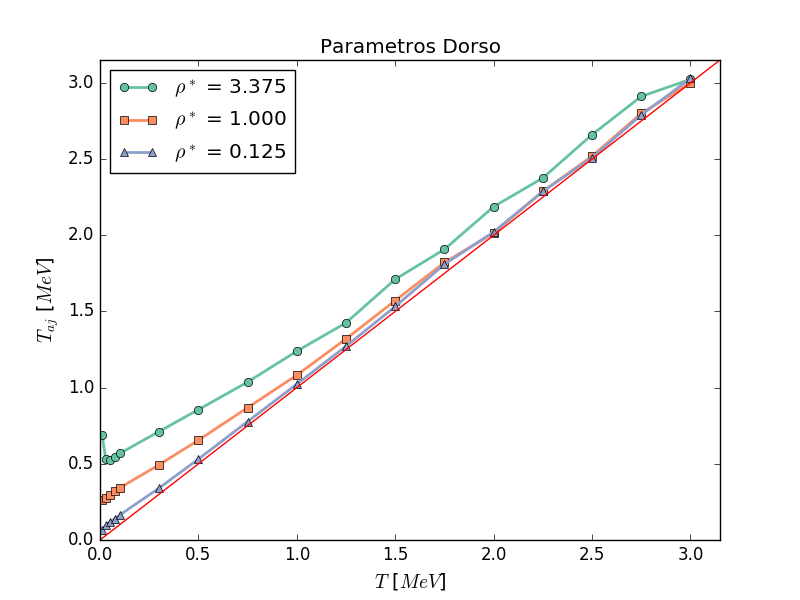
\includegraphics[trim = 5mm 0mm 20mm 5mm, clip, width=0.5\textwidth]{pauli_gas/TvsT_dorso.png}
	\caption{}
	\label{fig:TvsT_dorso}
\end{figure}

Con los histogramas obtenidos utilizando los parámetros de Maruyama \eqref{eq:params_maruyama} ocurre algo muy similar, como puede verse en las \textbf{Figuras \ref{fig:hist_rho0_maruyama}}, 
\textbf{\ref{fig:hist_rho1_maruyama}} y \textbf{\ref{fig:hist_rho2_maruyama}}.
Sin embargo, es ciertamente notable que la forma del histograma de los datos parece acompañar mejor a la distribución de FD y que los ajustes por FD resultan mucho más certeros, siendo
razonables para valores de $T$ considerablemente bajos.
Además, surge inmediatamente la diferencia de escalas entre temperaturas; las transiciones de las distribuciones del Pauli gas ocurren a $T$ un orden de magnitud mayor para estos parámetros.
Esto es llamativo y puede ciertamente estar asociado al hecho de que el $D^*$ mismo aumentó un orden de magnitud.

Esto ocurre en menor medida para la distribución de FD.
Es razonable que ocurra dado que, aunque los $\rho^*$ no cambiaron, si lo hicieron las densidades $\rho$ al cambiar el $q_o$.
Dado que el $q_o$ de Maruyama es menor, las densidades $\rho$ aumentaron, redefiniendo la noción de alta temperatura para valores de $T$ mayores.
Esto ciertamente nos muestra que el parámetro $q_o$ también influye a la hora de simular una distribución de FD vía un gas de Pauli.
\begin{figure}[H]
	\centering
	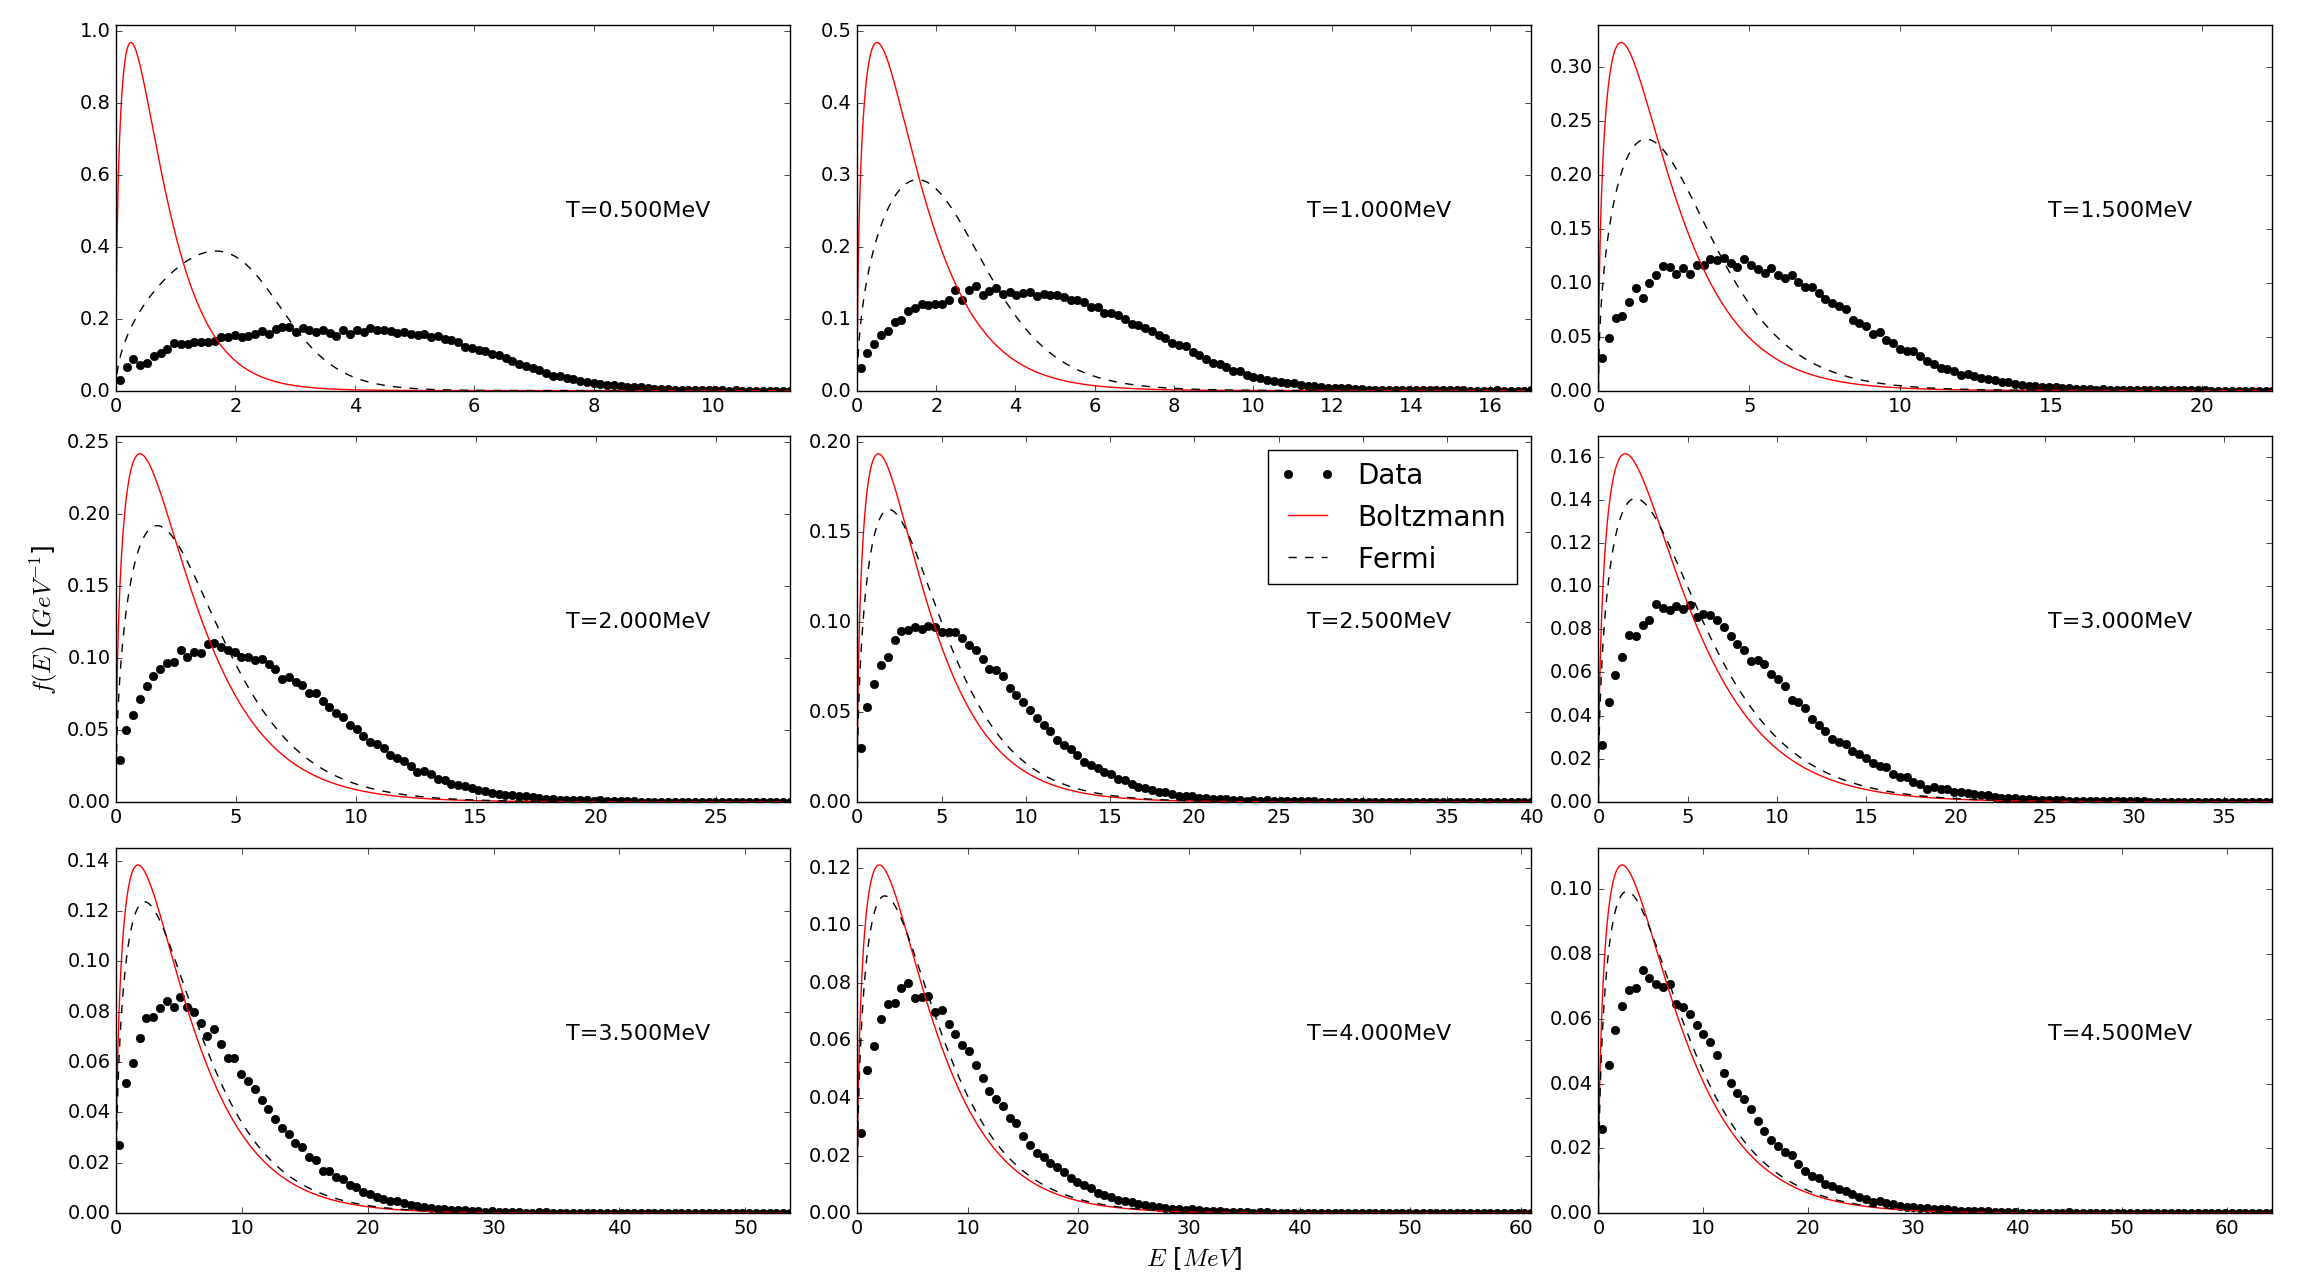
\includegraphics[width=0.9\textwidth]{pauli_gas/hist_rho0_maruyama.png}
	\caption{Distribuciones de energía cinética para los parámetros de Maruyama en \eqref{eq:params_maruyama} y $\rho^* = \rho_o^* = 3.375$}
	\label{fig:hist_rho0_maruyama}
\end{figure}
\begin{figure}[H]
	\centering
	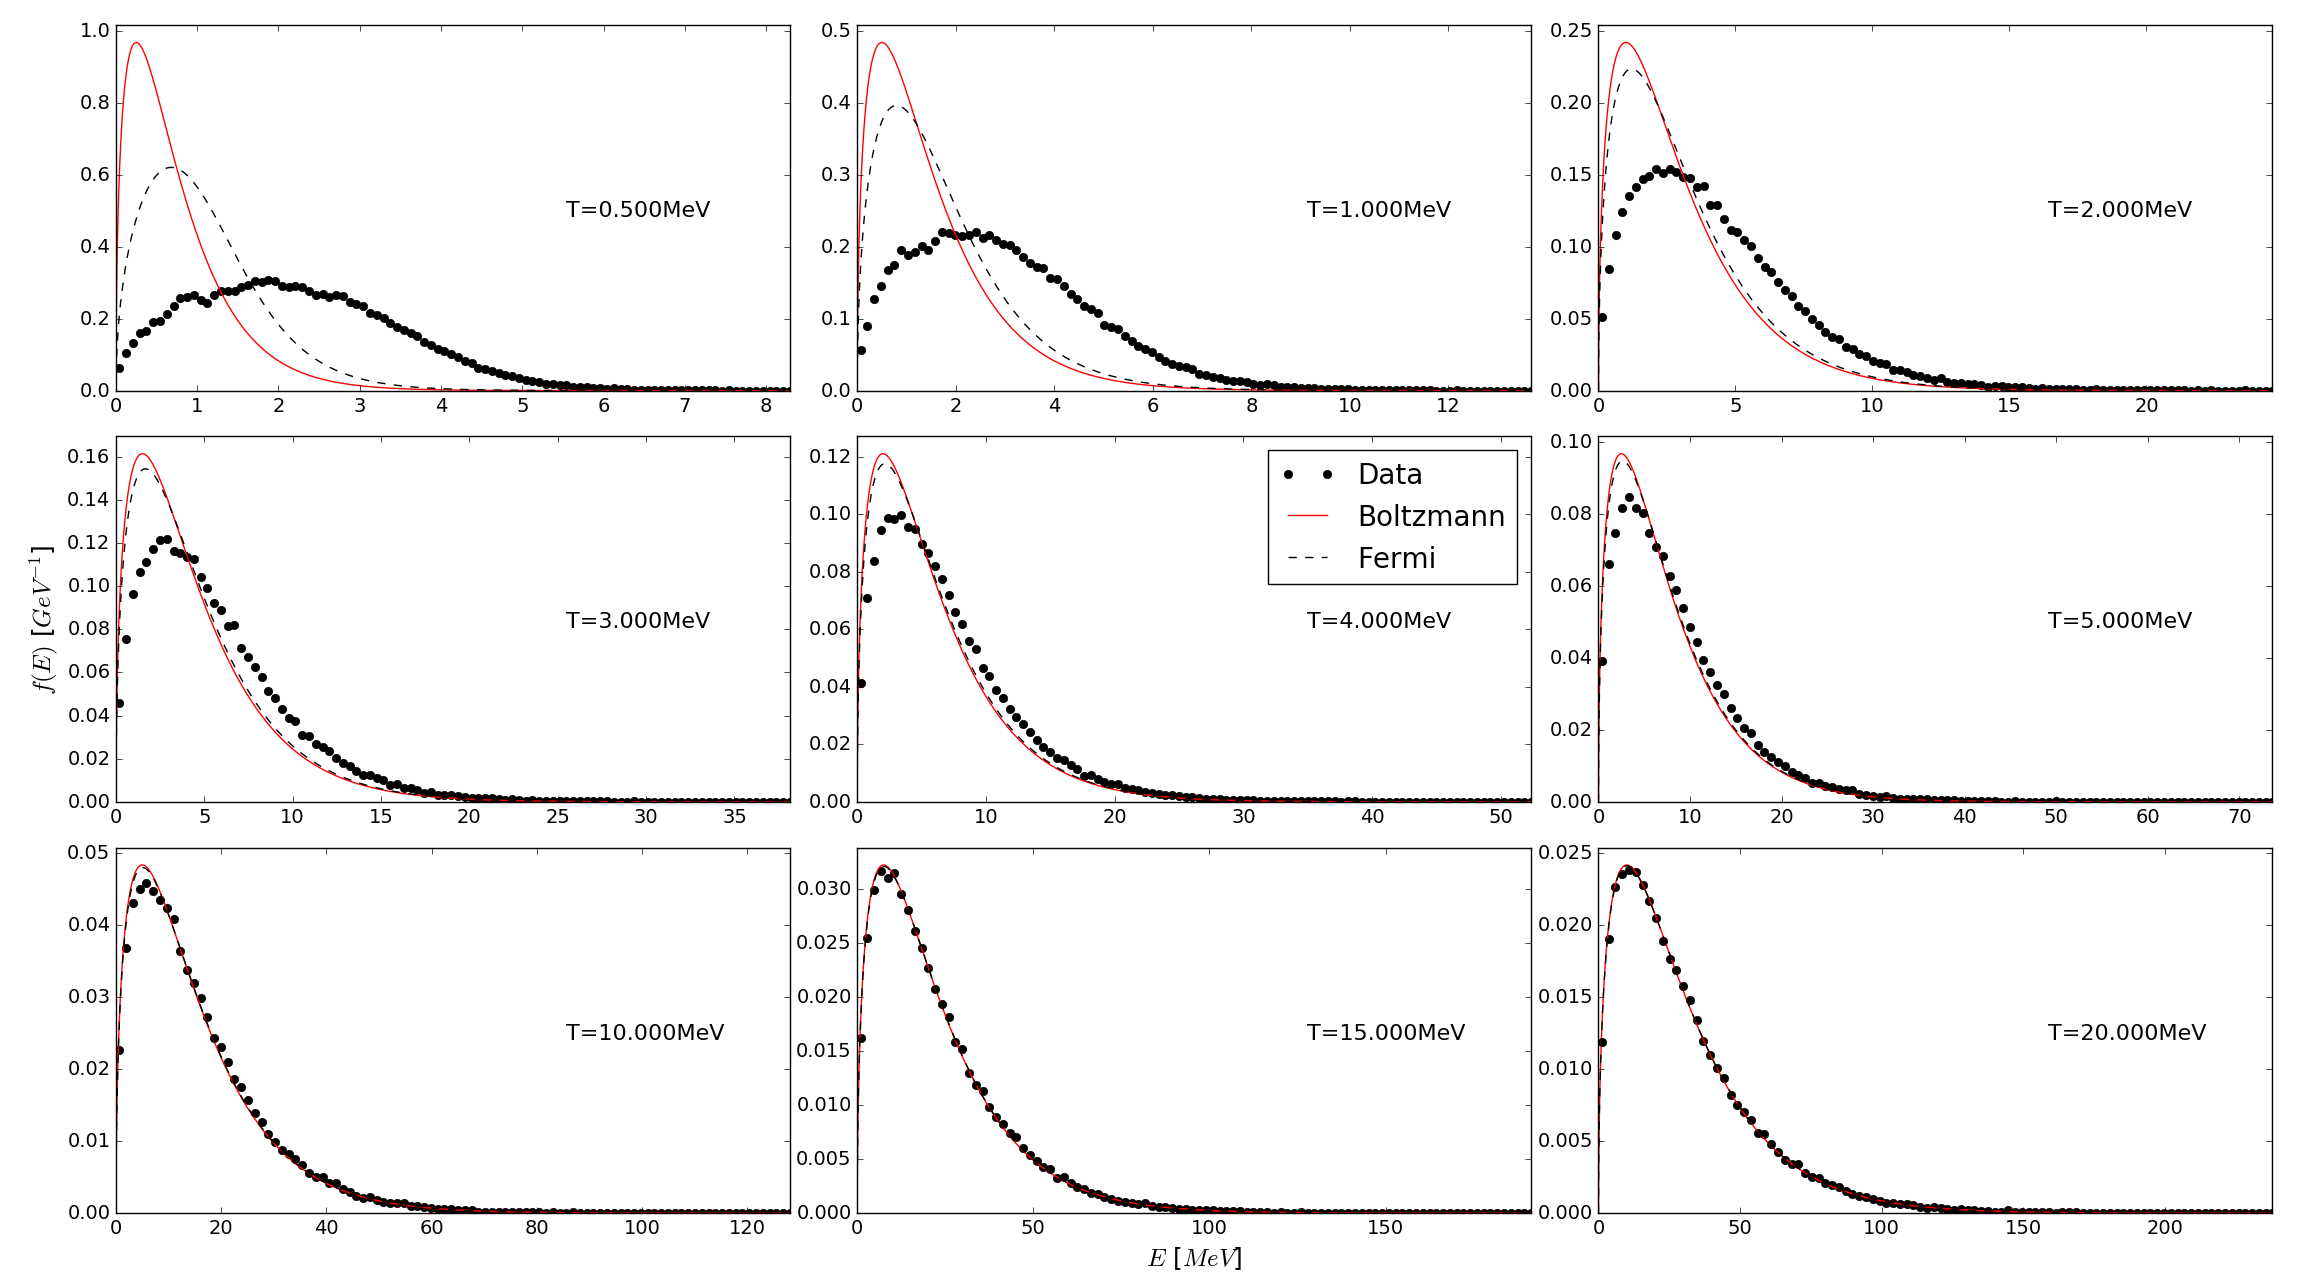
\includegraphics[width=0.9\textwidth]{pauli_gas/hist_rho1_maruyama.png}
	\caption{Distribuciones de energía cinética para los parámetros de Maruyama en \eqref{eq:params_maruyama} y $\rho^* = \rho_1^* = 1$}
	\label{fig:hist_rho1_maruyama}
\end{figure}
\begin{figure}[H]
	\centering
	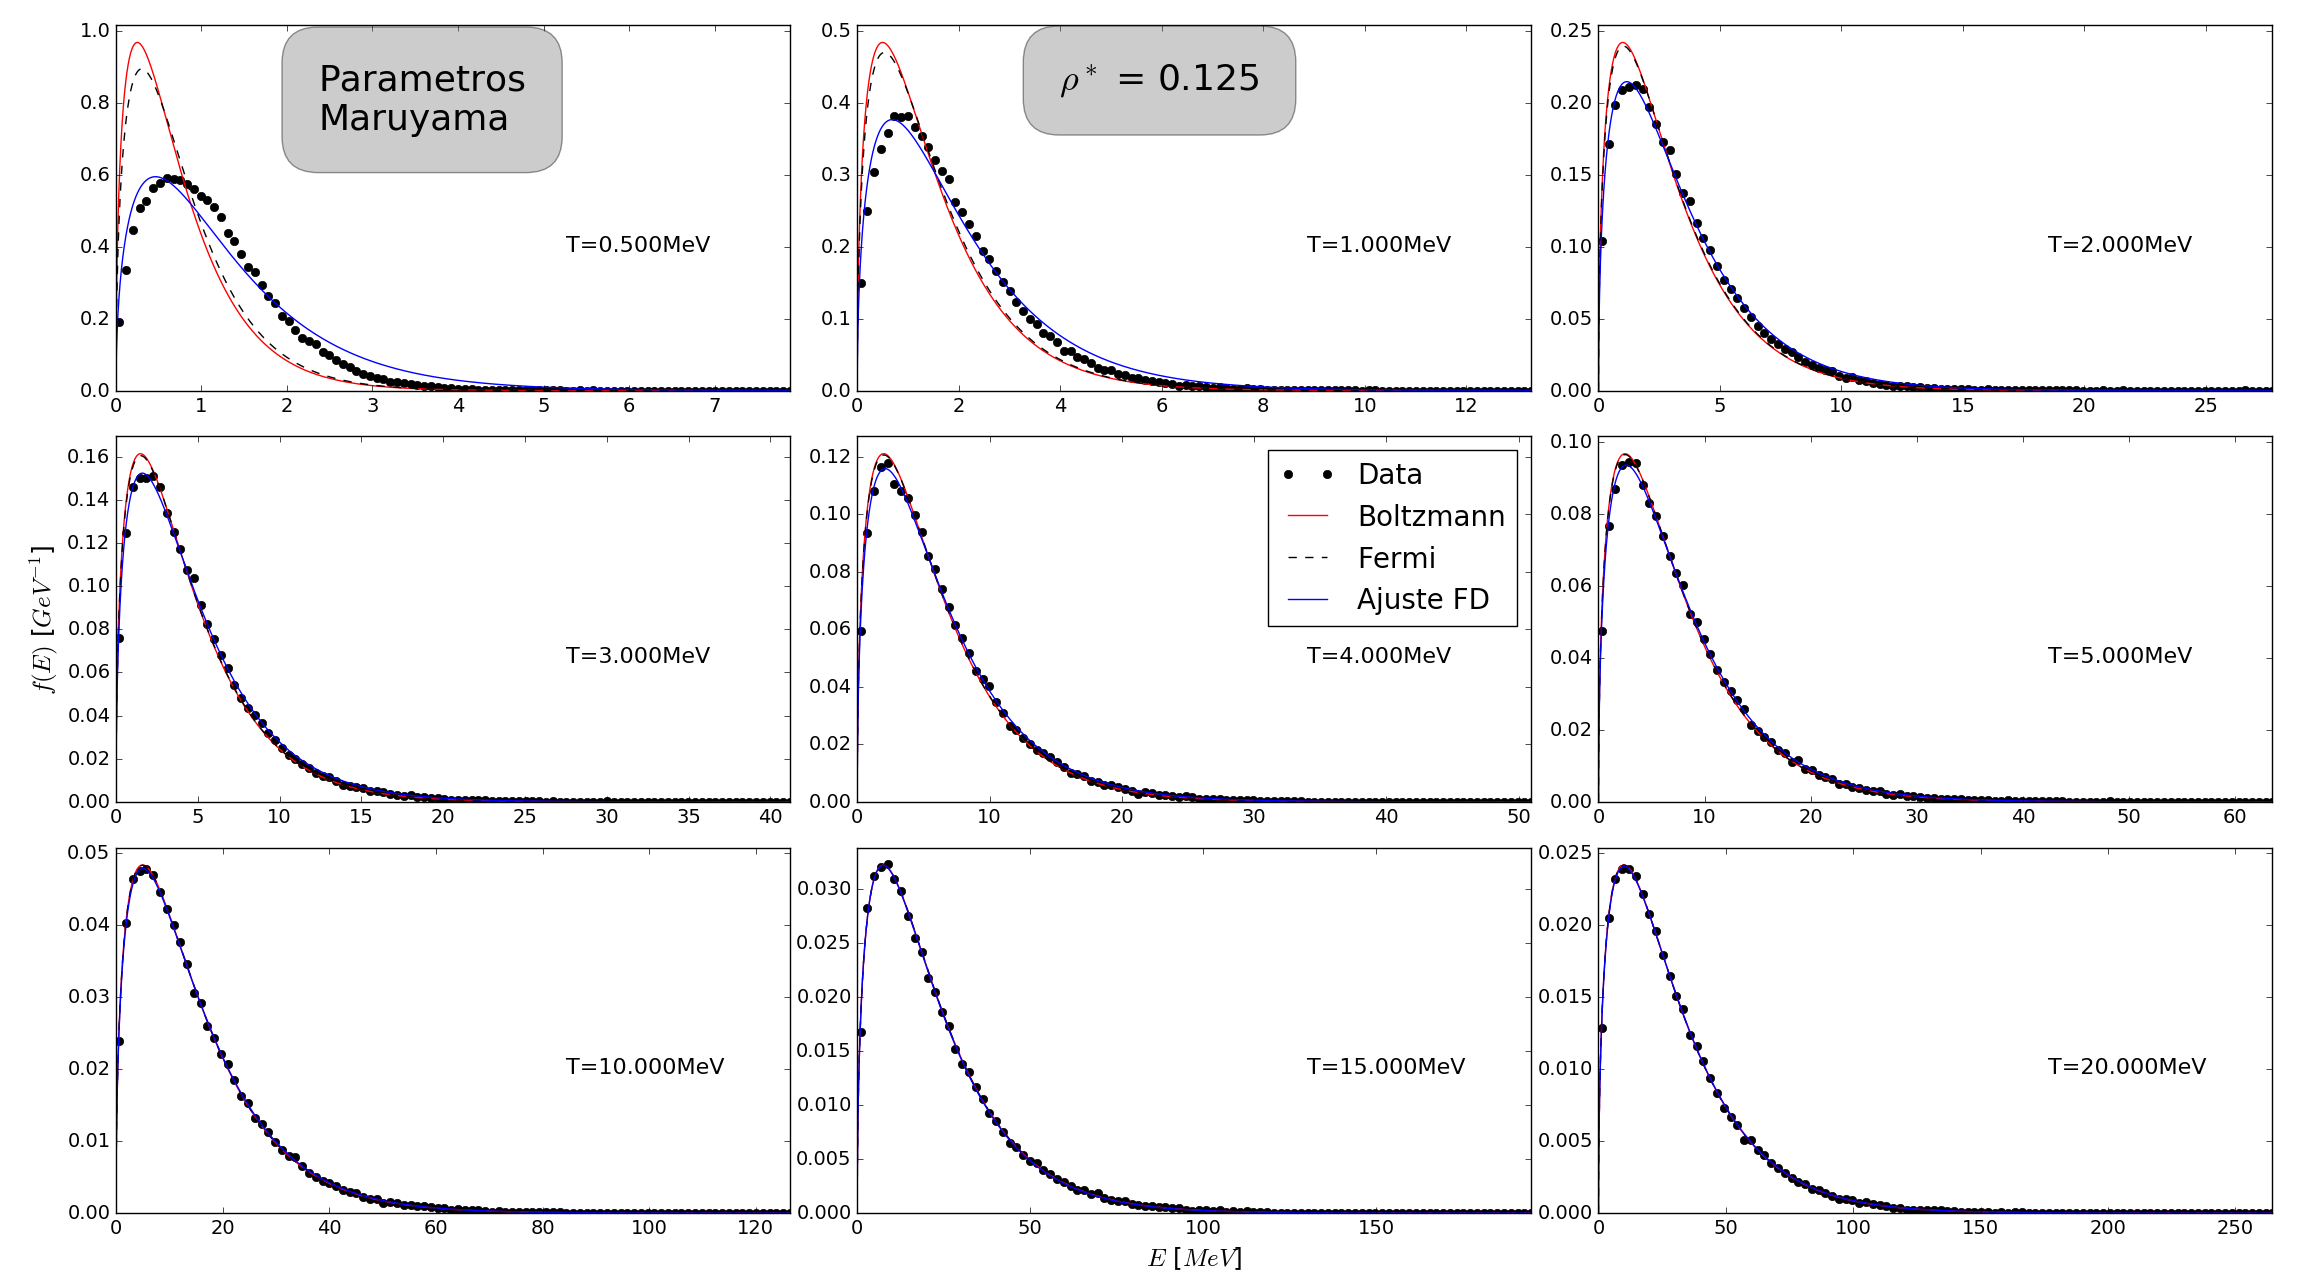
\includegraphics[width=0.9\textwidth]{pauli_gas/hist_rho2_maruyama.png}
	\caption{Distribuciones de energía cinética para los parámetros de Maruyama en \eqref{eq:params_maruyama} y $\rho^* = \rho_2^* = 0.125$}
	\label{fig:hist_rho2_maruyama}
\end{figure}

Nuevamente, los parámetros ajustados en comparación a los del FD exacto para esas condiciones se encuentran en las \textbf{Figuras \ref{fig:muvsT_dorso}} y \textbf{\ref{fig:TvsT_dorso}}.

\begin{figure}[H]
	\centering
	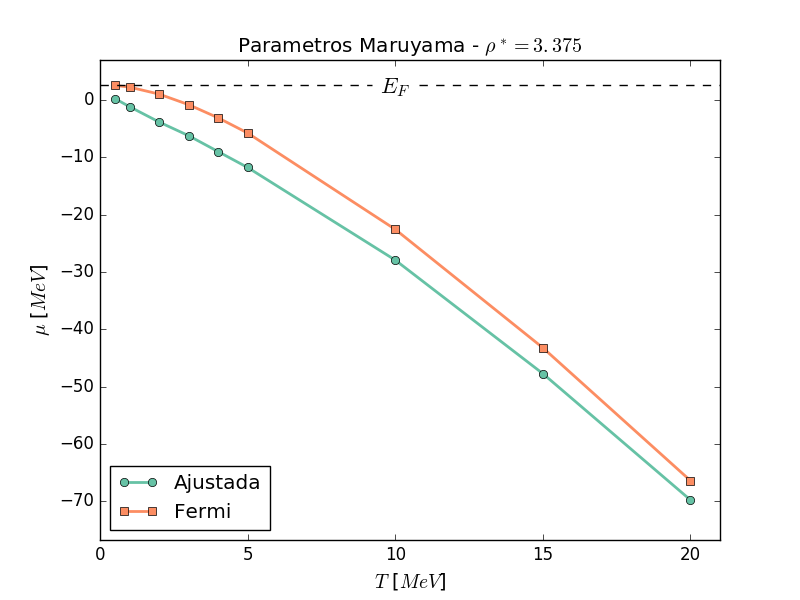
\includegraphics[trim = 5mm 0mm 20mm 5mm, clip, width=0.33\textwidth]{pauli_gas/muvsT_rho0_maruyama.png}
	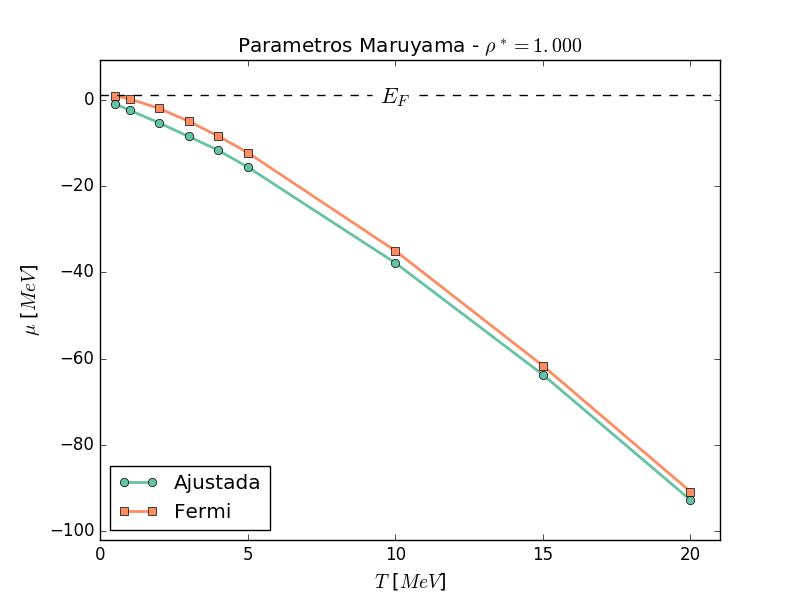
\includegraphics[trim = 5mm 0mm 20mm 5mm, clip, width=0.33\textwidth]{pauli_gas/muvsT_rho1_maruyama.png}
	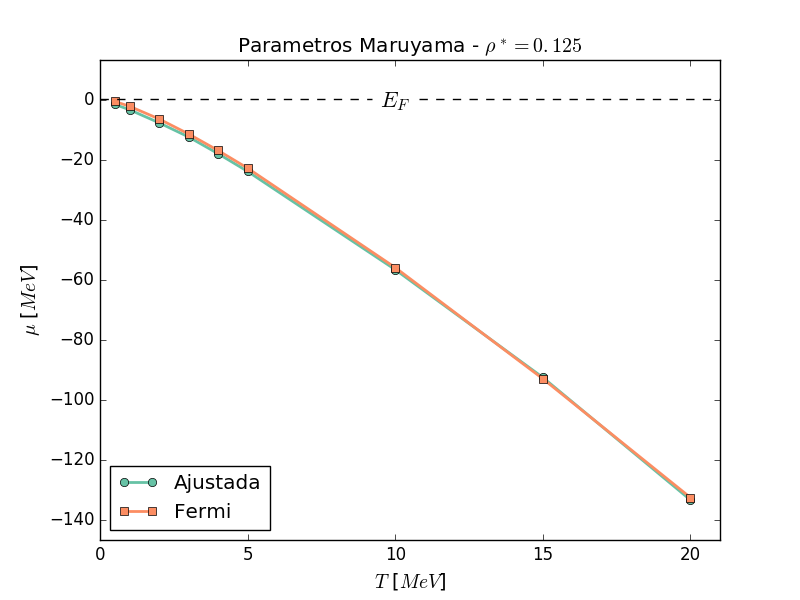
\includegraphics[trim = 5mm 0mm 20mm 5mm, clip, width=0.33\textwidth]{pauli_gas/muvsT_rho2_maruyama.png}
	\caption{}
	\label{fig:muvsT_maruyama}
\end{figure}
\begin{figure}[H]
	\centering
	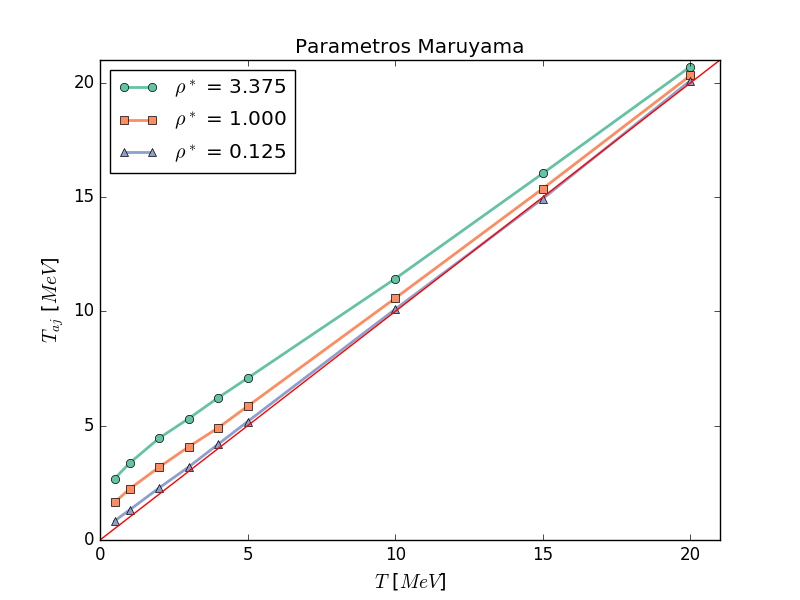
\includegraphics[trim = 5mm 0mm 20mm 5mm, clip, width=0.5\textwidth]{pauli_gas/TvsT_maruyama.png}
	\caption{}
	\label{fig:TvsT_maruyama}
\end{figure}

%%%%%%%%%%%%%%%%%%%%%%%%%%%%%%%%%%%%%%%%%%%%%%%%%%%%%%%%%%%%%%%%%%%%%%%%%%%%%%%%%%%%%%%%%%%%%%%%%%%%%%%%%%%%%%%%%%%%%%%%%%%%%%%%%%%%%%%%%%%%%%%%%%%%%%%%%%%%%%%%%%%%%%%%%%%%%%%%%%%%%%%%%%%%%

%Para entender esto, podemos nuevamente adimensionalizar el problema, analizando los parámetros que definen la forma de las distintas distribuciones.
%Dado que las distribuciones de energía cinética $f(\varepsilon)$ son extensivas, podemos obtener una magnitud intensiva del sistema dividiendolas por el número de partículas $N$.
%Esta nueva distribución intensiva solo puede depender de parámetros intensivos del sistema, como son la temperatura $T$ y la densidad $\rho$ pero también de parámetros microscópicos como
%la masa $m$ y la constante de Planck $\hbar$.
%Recordando las expresiones de $f_{FD}(\varepsilon)$ y $f_{MB}(\varepsilon)$ de \eqref{eq:dist_FD} y \eqref{eq:dist_MB}, vemos inmediatamente que podemos reescribir
%\[ f_{MB}(\varepsilon;N,T) = \frac{N}{T}g_{MB}(\varepsilon^*) \]
%\[ f_{FD}(\varepsilon;N, V, T, m, \hbar) = \frac{N}{T}g_{FD}(\varepsilon^*;\lambda^3\rho) \]
%donde $\varepsilon^* = \varepsilon/T$ y $\lambda$ es la longitud de onda términa previamente definida.
%En resumen, la adimensionalización nos permite eliminar 3 variables, mientras que la linealidad en $N$ nos permite eliminar una cuarta.
%
%Podemos hacer un razonamiento análogo para la distribución $f_P(\varepsilon)$ de un gas de Pauli.
%Los parámetros relevantes siguen siendo $T$, $\rho$ y $m$ pero también se suman los $D$, $q_o$ y $p_o$ del potencial de Pauli.
%Una adimensionalización como la de \ref{sec:adim_choque1d} arrojaría inmediatamente 
%\[ f_P(\varepsilon; N,V,T, m D, q_o,p_o.) = \frac{N}{T}g_P(\varepsilon^*; D^*, T^*, \rho^*)\]
%con la definición habitual $D^*=Dm/p_o^2$, $T^*=Tm/p_o^2$ y $\rho^* = \rho q_o^3$.
%
%Bajo estas consideraciones, la única diferencia entre la $f_P$ obtenida con los distintos parámetros para Pauli se debe $D^*$ y $T^*$ (pues mantuvimos $\rho^*$); a los parámetros $D$ y $p_o$.
%Sin embargo, la similitud entre $f_P$ y $f_{FD}$ cambia pues $f_{FD}$ depende de $\rho$ en lugar de $\rho^*$, reescalando las temperaturas.
%Esto en principio parecería indicar que todos los parámetros del potencial de Pauli son relevantes a la hora de emular la distribución de FD.
%
%Esto último resulta razonable si consideramos que la forma de la región excluída también es relevante para el problema.
%Su forma resulta basicamente elíptica, pero los parámetros $q_o$ y $p_o$ regulan sus ejes.
%Sin embargo, a priori no es posible afirmar que estos parámetros $D$, $q_o$ y $p_o$ puedan ser independientes de la temperatura $T$ y $\rho$.
%Esto ciertamente es deseable, pero un estudio pormenorizado de estas cuestiones excede el alcance de este trabajo.

%%%%%%%%%%%%%%%%%%%%%%%%%%%%%%%%%%%%%%%%%%%%%%%%%%%%%%%%%%%%%%%%%%%%%%%%%%%%%%%%%%%%%%%%%%%%%%%%%%%%%%%%%%%%%%%%%%%%%%%%%%%%%%%%%%%%%%%%%%%%%%%%%%%%%%%%%%%%%%%%%%%%%%%%%%%%%%%%%%%%%%%%%%%%%

Por último, mostramos en las \textbf{Figuras \ref{fig:hist_rho0_LJ}} y \textbf{\ref{fig:hist_rho1_LJ}} las distribuciones de energía cinética obtenidas para un gas de LJ.
En contraposición a lo anterior, su distribución resulta idénticamente la de MB.

\begin{figure}[H]
	\centering
	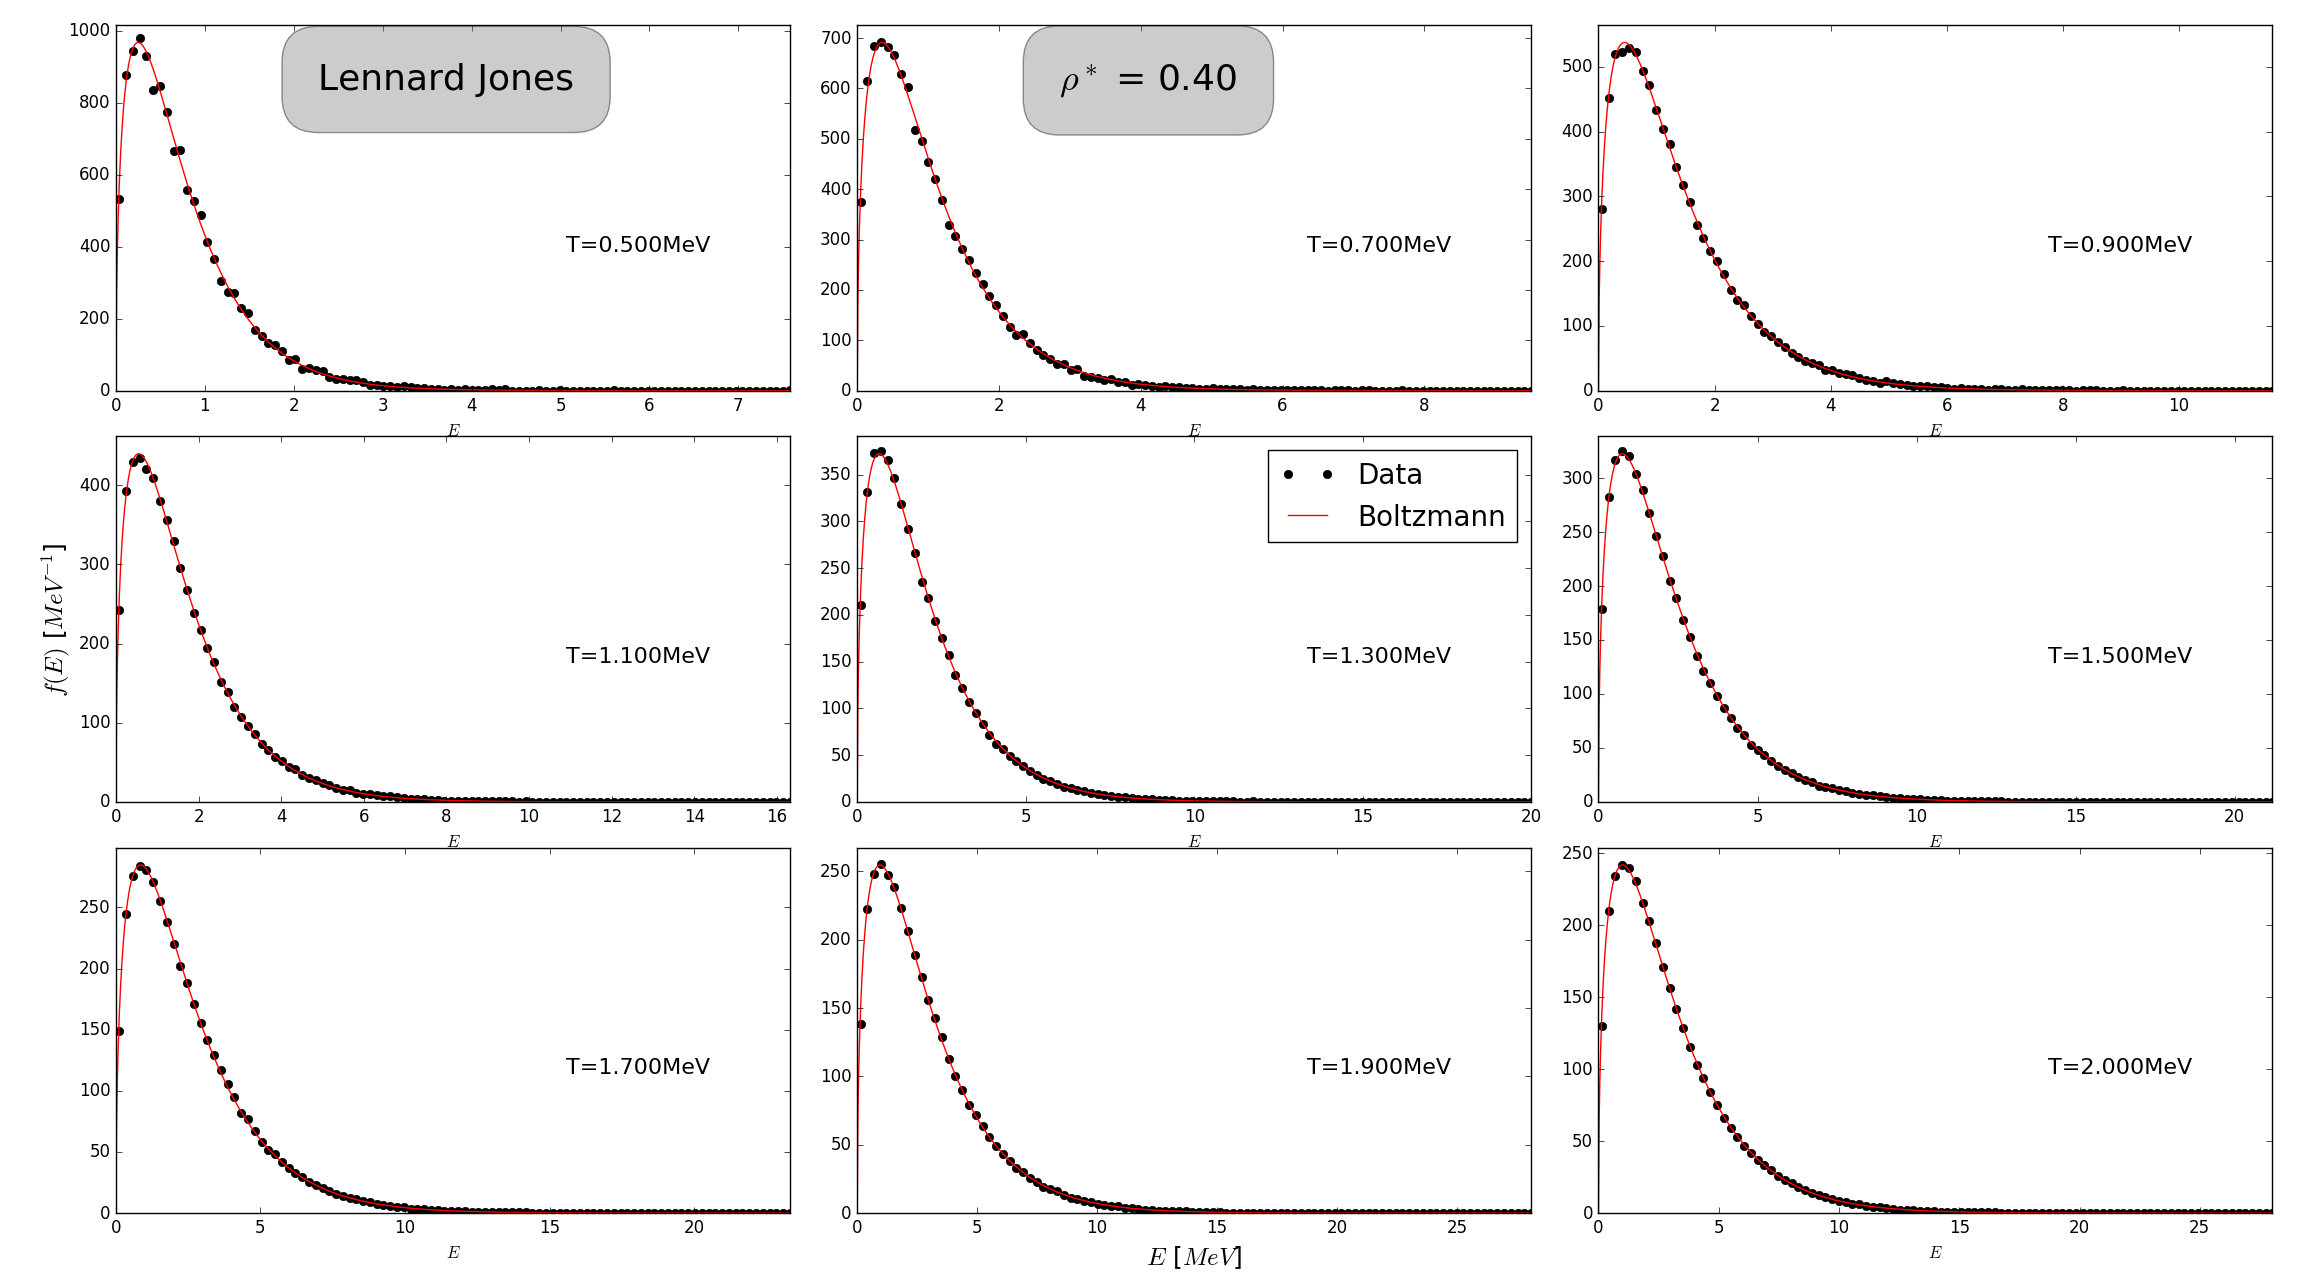
\includegraphics[width=0.9\textwidth]{pauli_gas/hist_rho0_LJ.png}
	\caption{Distribuciones de energía cinética para gas de Lennard Jones y $\rho^* = 0.4$.
	La distribución resulta inequivocamente Maxwell-Boltzmann.}
	\label{fig:hist_rho0_LJ}
\end{figure}

\begin{figure}[H]
	\centering
	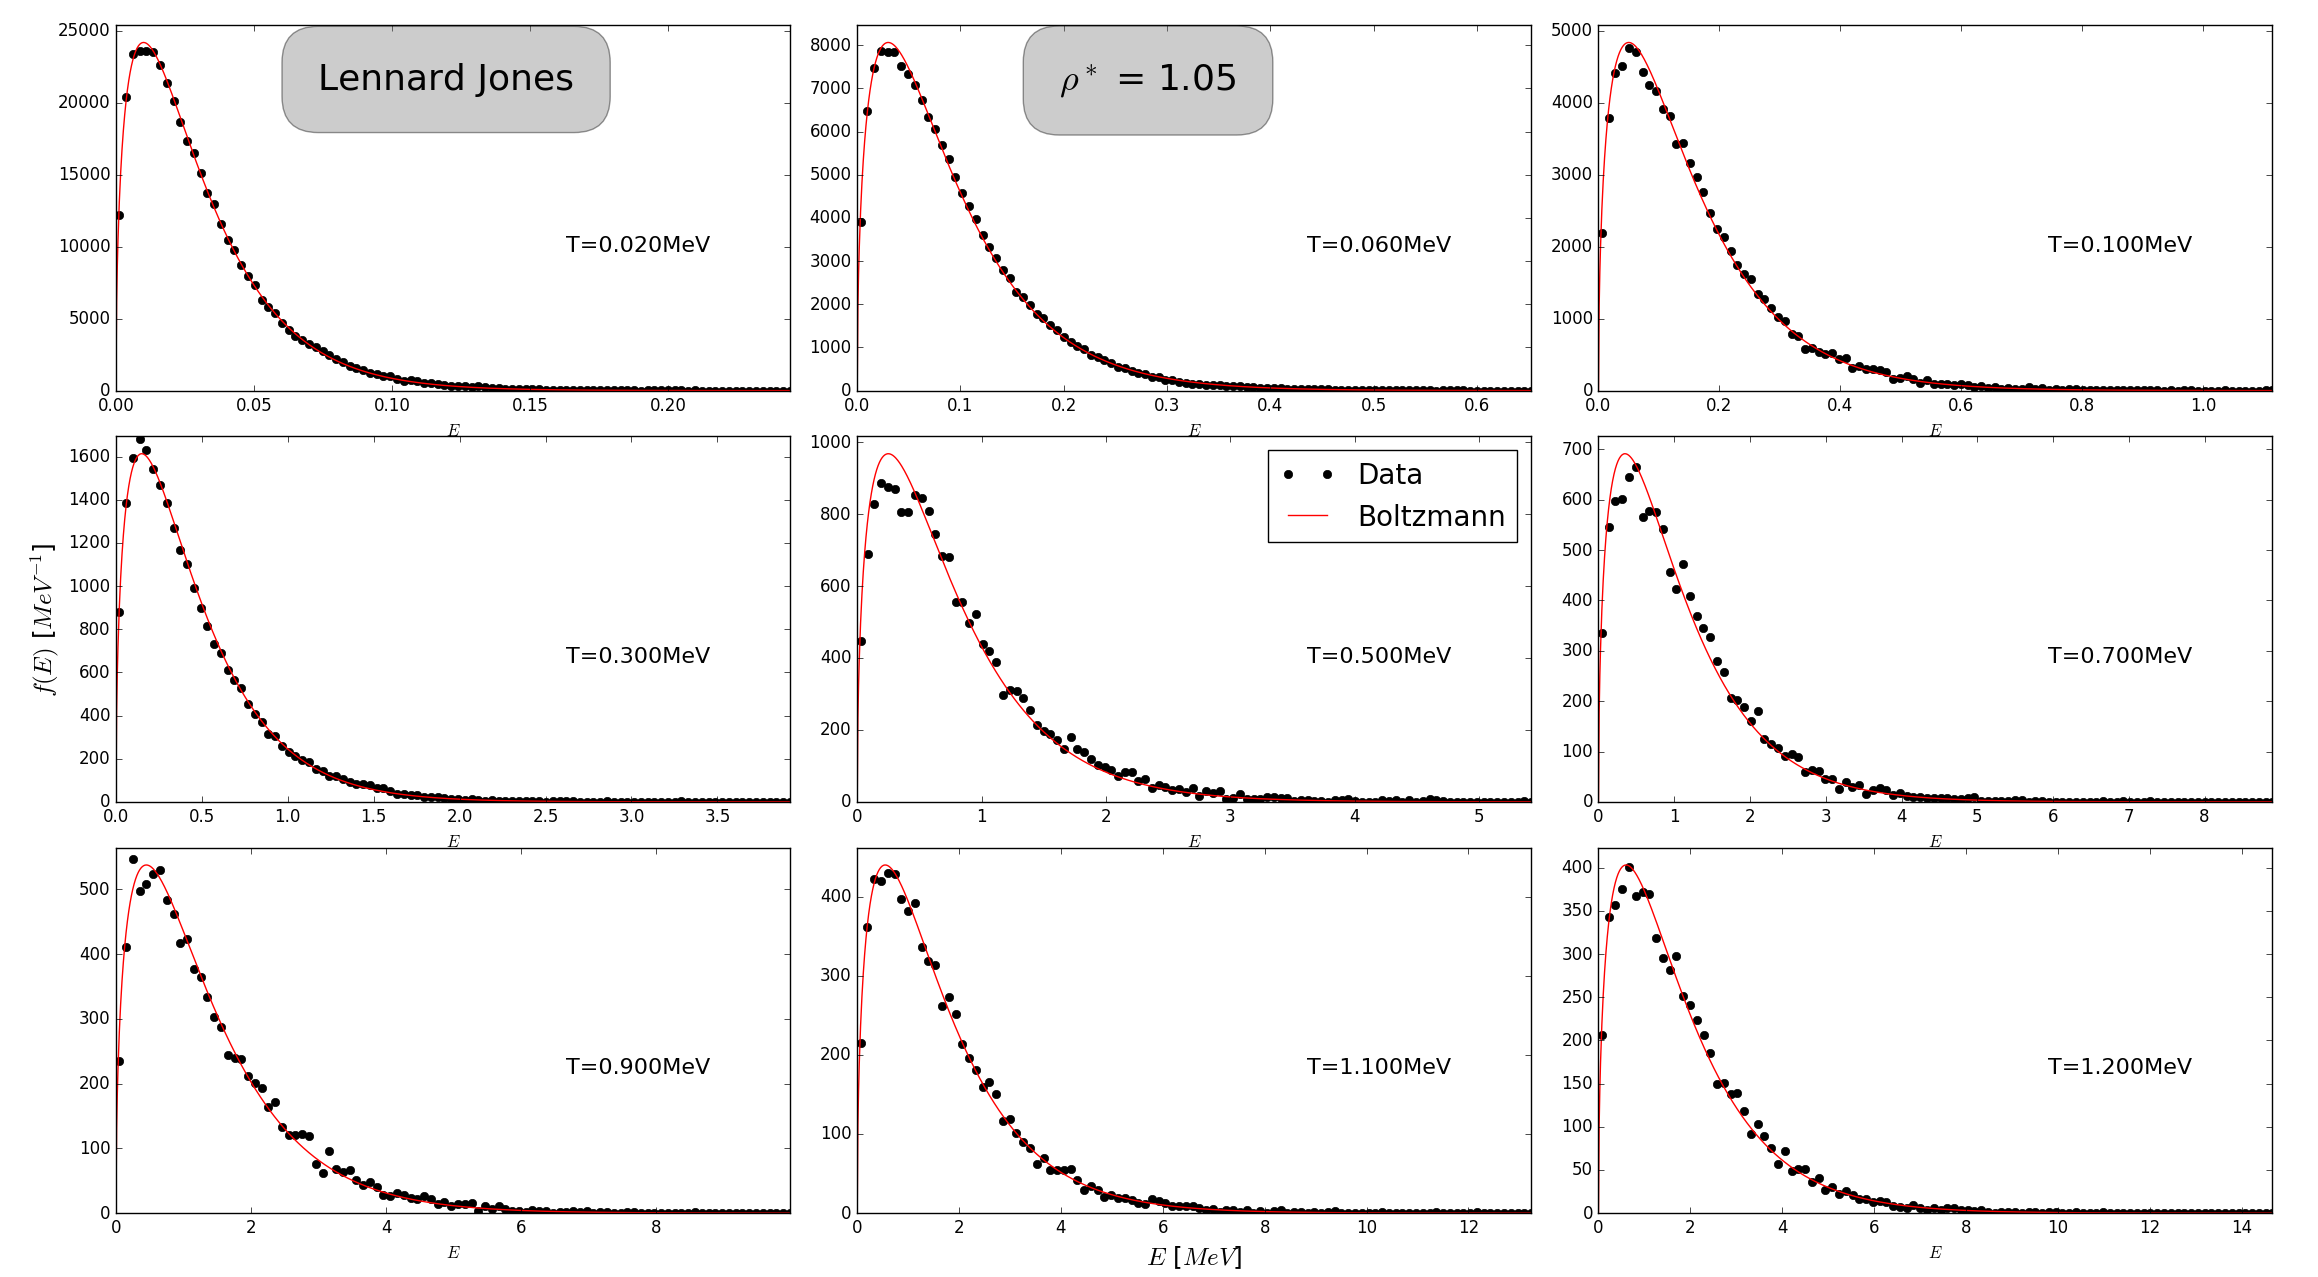
\includegraphics[width=0.9\textwidth]{pauli_gas/hist_rho1_LJ.png}
	\caption{Distribuciones de energía cinética para gas de Lennard Jones y $\rho^* = 1.05$.
	La distribución resulta inequivocamente Maxwell-Boltzmann.}
	\label{fig:hist_rho1_LJ}
\end{figure}


\subsection{Area excluída}



\begin{figure}[H]
	\centering	%trim={<left> <lower> <right> <upper>}
	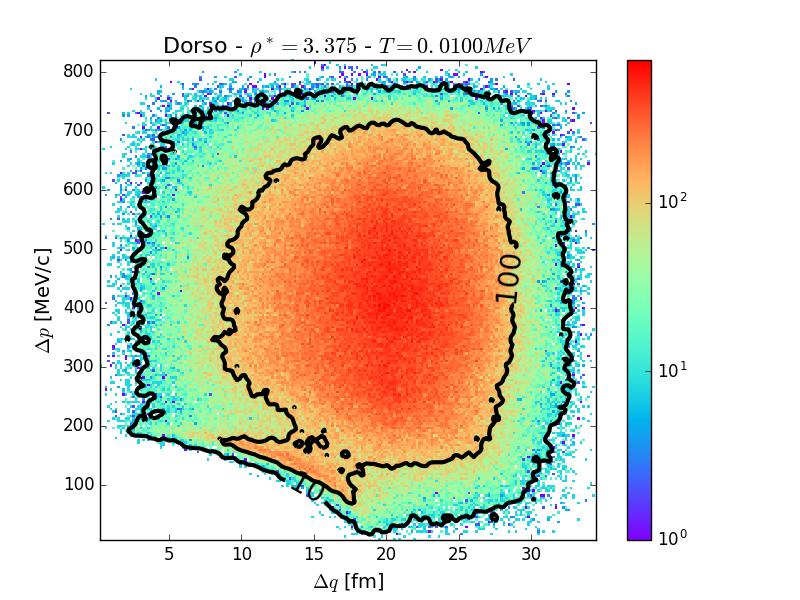
\includegraphics[trim = 5mm 0mm 50mm 5mm, clip, height=0.3\textwidth]{pauli_gas/exclusion_rho0_dorso_0,01.png}
	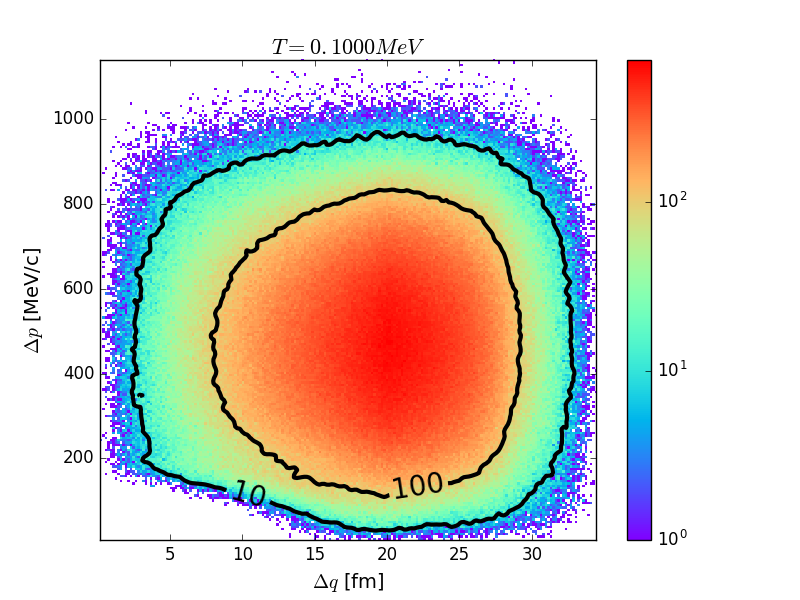
\includegraphics[trim = 25mm 0mm 50mm 5mm, clip, height=0.3\textwidth]{pauli_gas/exclusion_rho0_dorso_0,1.png}
	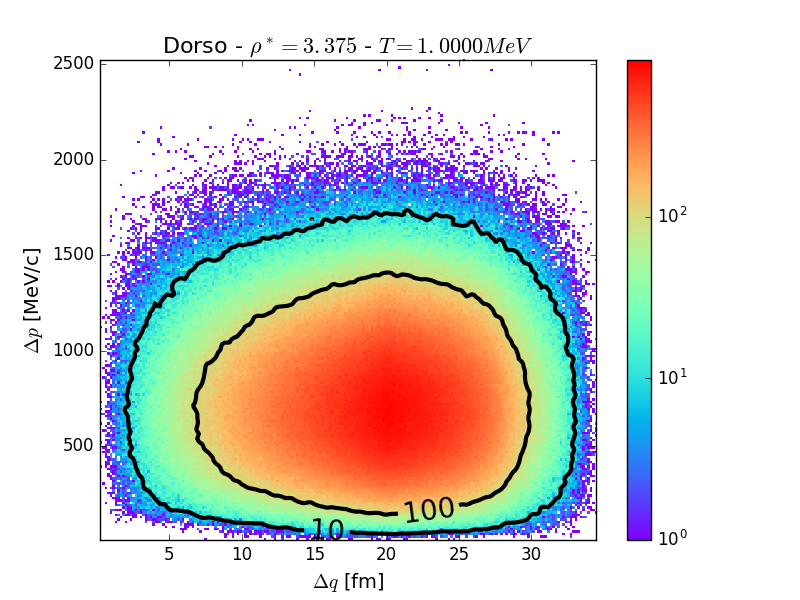
\includegraphics[trim = 25mm 0mm 20mm 5mm, clip, height=0.3\textwidth]{pauli_gas/exclusion_rho0_dorso_1.png}
	\caption{}
	\label{fig:exclusion_rho0_dorso}
\end{figure}

\begin{figure}[H]
	\centering	%trim={<left> <lower> <right> <upper>}
	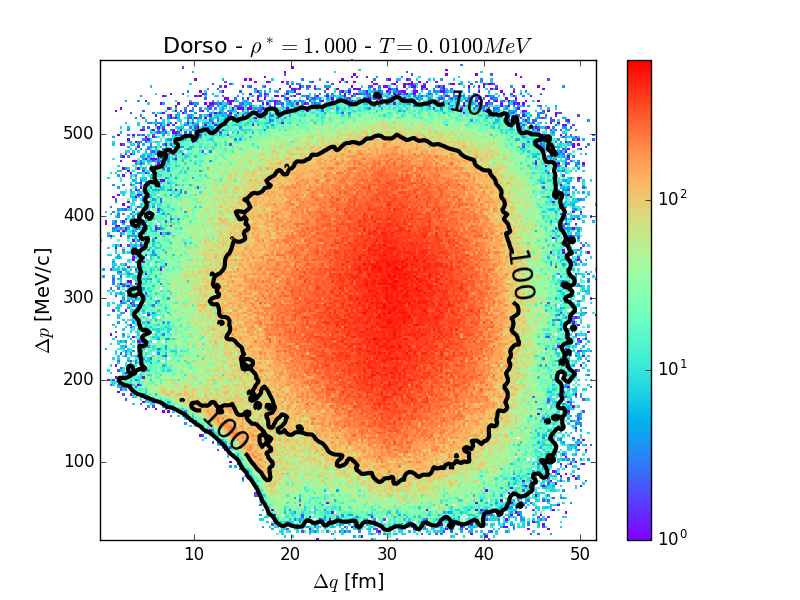
\includegraphics[trim = 5mm 0mm 50mm 5mm, clip, height=0.3\textwidth]{pauli_gas/exclusion_rho1_dorso_0,01.png}
	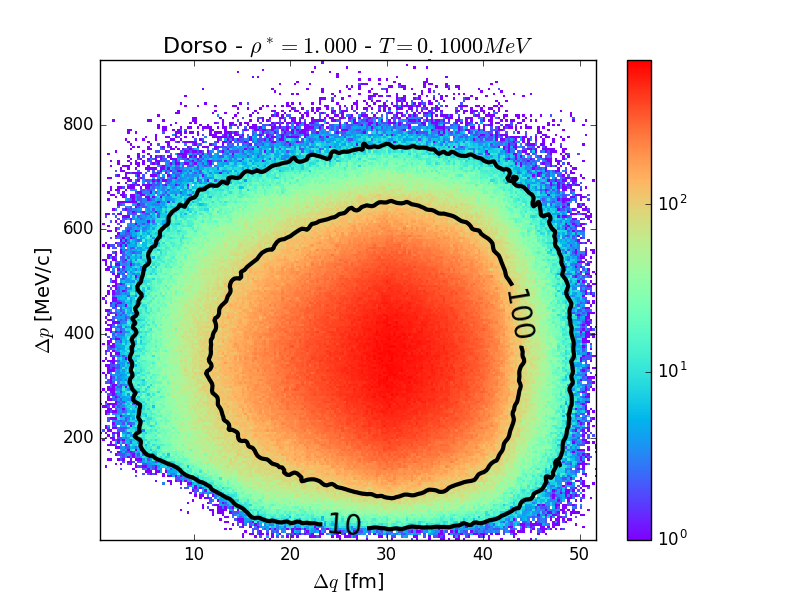
\includegraphics[trim = 25mm 0mm 50mm 5mm, clip, height=0.3\textwidth]{pauli_gas/exclusion_rho1_dorso_0,1.png}
	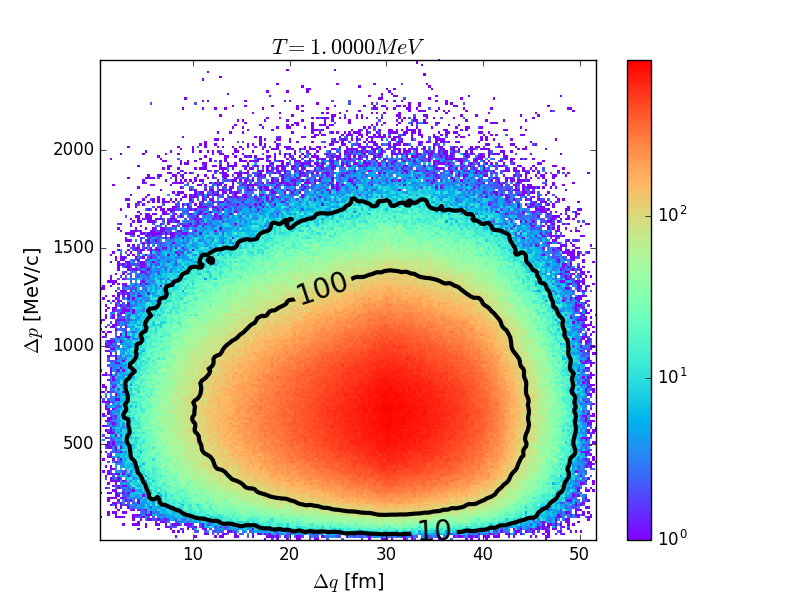
\includegraphics[trim = 25mm 0mm 20mm 5mm, clip, height=0.3\textwidth]{pauli_gas/exclusion_rho1_dorso_1.png}
	\caption{}
	\label{fig:exclusion_rho1_dorso}
\end{figure}

\begin{figure}[H]
	\centering	%trim={<left> <lower> <right> <upper>}
	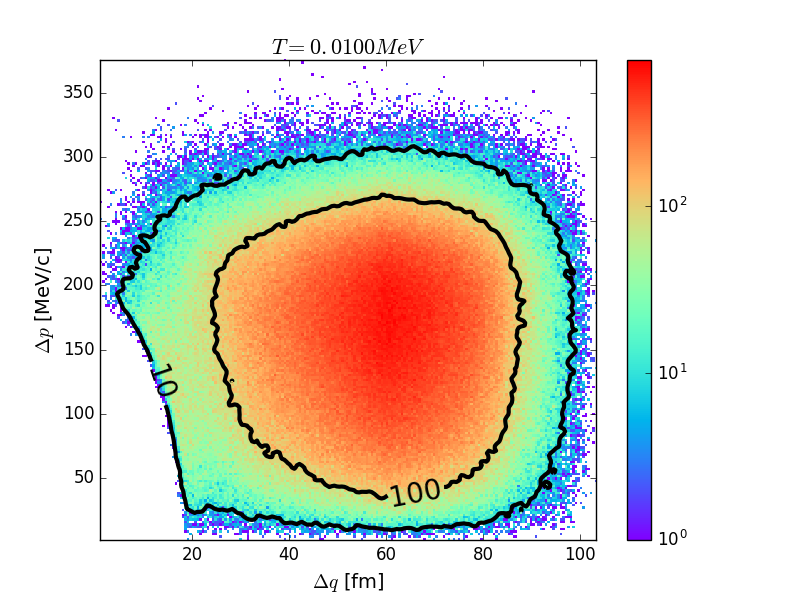
\includegraphics[trim = 5mm 0mm 50mm 5mm, clip, height=0.3\textwidth]{pauli_gas/exclusion_rho2_dorso_0,01.png}
	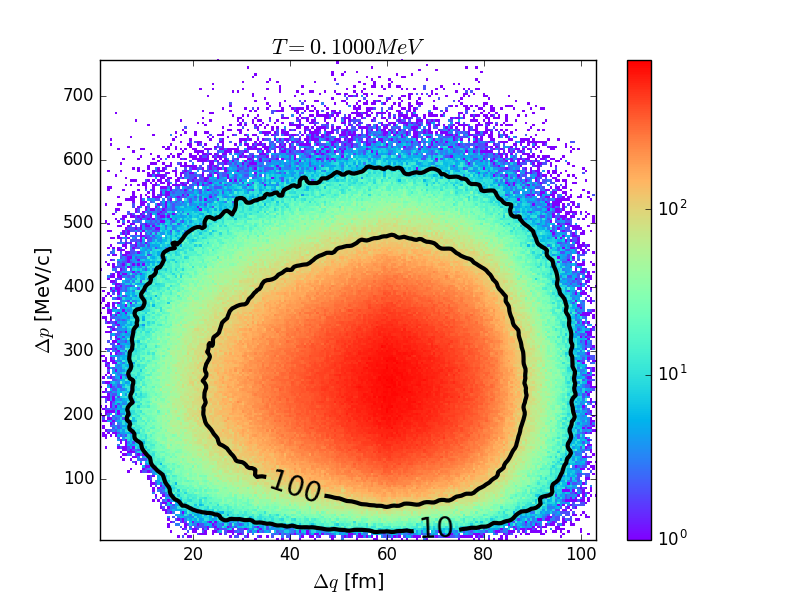
\includegraphics[trim = 25mm 0mm 50mm 5mm, clip, height=0.3\textwidth]{pauli_gas/exclusion_rho2_dorso_0,1.png}
	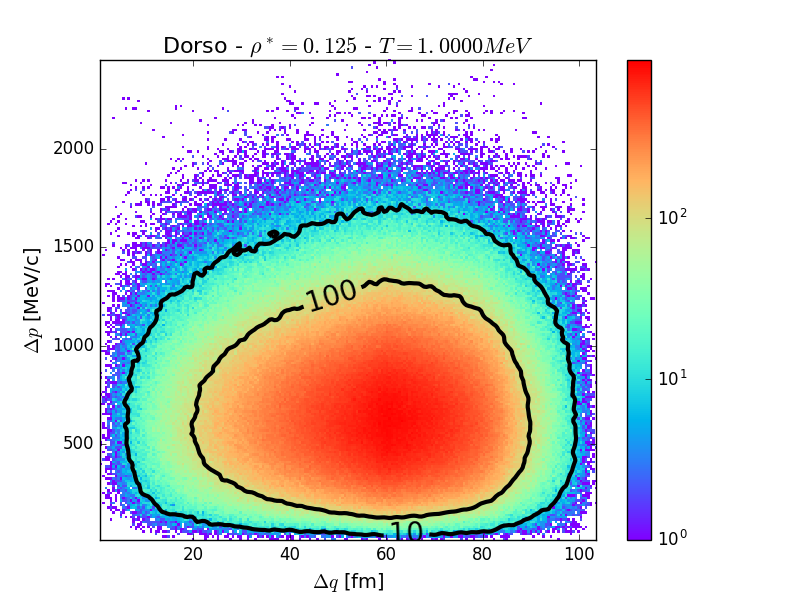
\includegraphics[trim = 25mm 0mm 20mm 5mm, clip, height=0.3\textwidth]{pauli_gas/exclusion_rho2_dorso_1.png}
	\caption{}
	\label{fig:exclusion_rho2_dorso}
\end{figure}

\begin{figure}[H]
	\centering	%trim={<left> <lower> <right> <upper>}
	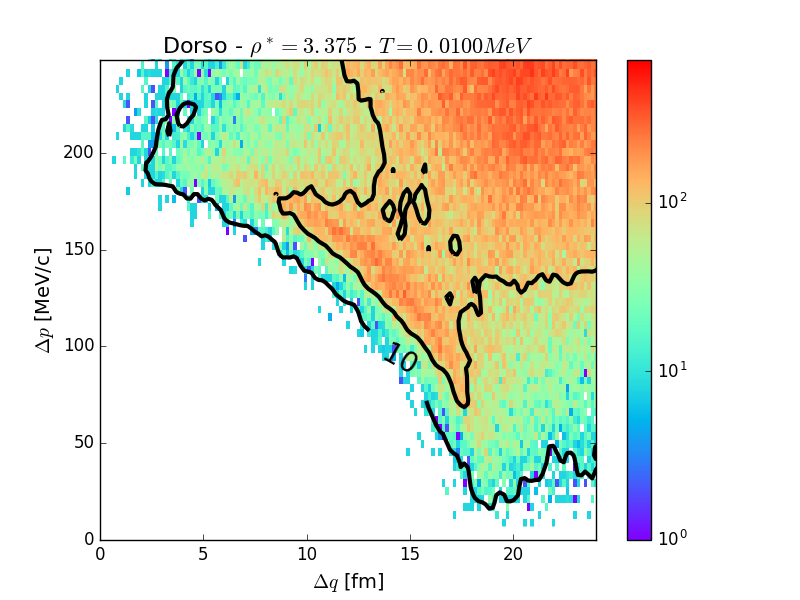
\includegraphics[trim = 5mm 0mm 50mm 5mm, clip, height=0.3\textwidth]{pauli_gas/exclusion_zoom_rho0_dorso_0,01.png}
	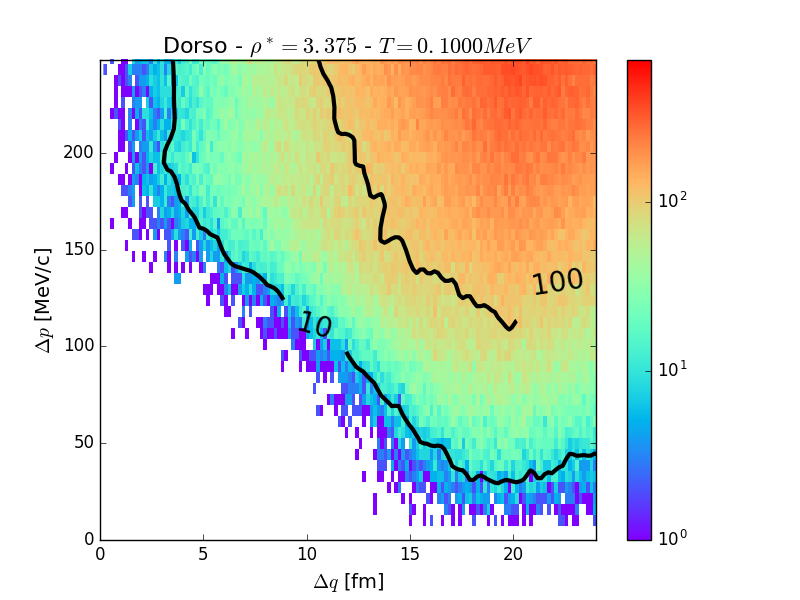
\includegraphics[trim = 25mm 0mm 50mm 5mm, clip, height=0.3\textwidth]{pauli_gas/exclusion_zoom_rho0_dorso_0,1.png}
	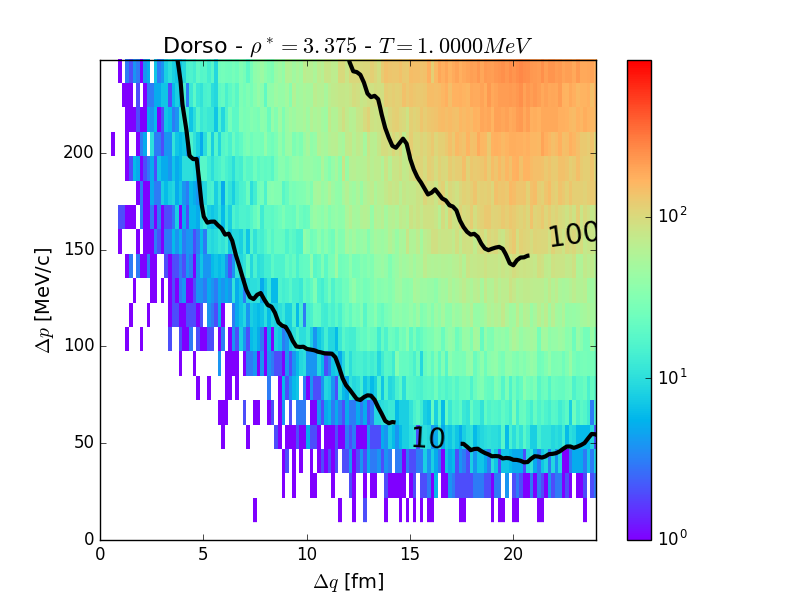
\includegraphics[trim = 25mm 0mm 20mm 5mm, clip, height=0.3\textwidth]{pauli_gas/exclusion_zoom_rho0_dorso_1.png}
	\caption{}
	\label{fig:exclusion_zoom_rho0_dorso}
\end{figure}

\subsection{Presión}